% \documentclass[11pt,twoside,a4paper]{article}
% \usepackage{times}

% \usepackage{xeCJK}

% \setmainfont{Times New Roman}

% \setCJKmainfont{Songti SC}
\documentclass[10pt]{ctexart}
% \usepackage[UTF-8]{ctex}
\usepackage{amsmath}
\usepackage{amssymb}  %为了能使用\mathbb{H} 
\usepackage{booktabs}
\usepackage{multirow}
\usepackage{tabularx}
\usepackage{color}
\usepackage[colorlinks,linkcolor=blue]{hyperref} % 使用超链接
\usepackage{pdfpages}
\usepackage{geometry}
\geometry{a4paper,scale=0.8}
\usepackage{graphicx} %插入图片的宏包
\usepackage{float} %设置图片浮动位置的宏包
\usepackage{subfigure} %插入多图时用子图显示的宏包

\newtheorem{definition}{定义}
\newtheorem{lemma}{引理}
\newtheorem{theorem}{定理}


\title{区块链技术与应用}
\author{谢文进}
\date{\today}
\begin{document}
\maketitle
\tableofcontents
\section{课程简介}

\includepdf[pages=2-6,nup=1x2]{01.pdf} 
\section{BTC-密码学原理}
加密货币(Crypto-currency)中主要用到密码学中的哈希函数和签名。
\subsection{哈希函数}
哈希函数(hash function)有两个性质:
\begin{itemize}
    \item \textbf{collision resistance (or collision free)}:不能在多项式时间内找到$x \neq y$,使得$H(x)=H(y)$。这条性质说明没有办法篡改内容而又不被检测出来。
    \item \textbf{hiding}:$x \rightarrow H(x)$是单向的,不可逆的。这里有个前提是要求输入空间大,取值分布均匀。
\end{itemize}
没有哪个哈希函数在数学上证明是collision resistance的,但是可以找到哈希碰撞的方法,例如MD5就被攻破了。

可以用哈希函数的hiding性质做digital commitment, 也就是digital equivalent of a sealed envelope。比如预测股市,先将结果放在信封里,不能提前公布预测结果,因为预测的结果可能会影响股市,接着将信封交给第三方保证不被篡改,等到开盘再打开验证。如果使用哈希函数,可以先公布哈希值$H(x)$,等到要验证时,再拿出之前写好的$x$。哈希函数hiding性质的前提是输入要足够大,分布均匀,如果输入不够大,可以在$x$后面拼接随机数$H(x||nonce)$。

bitcoin中还要求哈希函数有\textbf{puzzle friendly}性质。由于哈希值的计算事先是不可预测的,可以设置一个puzzle,比如要求计算出的哈希值前$k$个都为0,形如$00\cdots 0 $xx$\cdots$x。这其实就是挖矿,找一个随机数nonce,使得H(block header) $\le$ target,block header中含有可调节的nonce。
\begin{figure}[H]
    \centering
    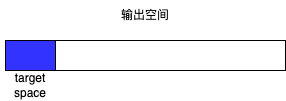
\includegraphics[width=0.4\textwidth]{./lecture2/lecture1-1.png} 
\end{figure}
输出空间很大,但是目标空间很小,这只能一个一个试nonce的值。这也是工作量证明(proof of work)。虽然挖矿很难,但是验证比较容易(difficult to solve, but easy to verify)。
\subsection{签名}
在比特币中开户其实就是创建一个\textbf{公私钥对}(public key, private key)。公钥相当于银行账户,私钥相当于密码。在进行交易时,用私钥进行签名,说明是本人进行的,发布交易时也要发送公钥,可供他人进行验证。

在这个过程中,产生公私钥对和签名时需要一个好的随机源(a good source of randomness)。
\section{BTC-数据结构}
\subsection{哈希指针}
hash pointer
\begin{figure}[H]
    \centering
    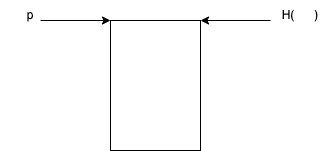
\includegraphics[width=0.4\textwidth]{./lecture3/img1.png} 
\end{figure}
Block chain is a linked list using hash pointer.
\begin{figure}[H]
    \centering
    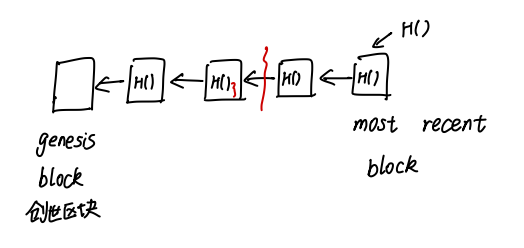
\includegraphics[width=0.5\textwidth]{./lecture3/img2.png} 
\end{figure}

实现\textbf{tamper-evident log},只要保存最后一个值,就知道前面有没有修改。
\subsection{Merkle tree}
Merkle tree是用Hash指针代替普通指针的二叉树。
\begin{figure}[H]
    \centering
    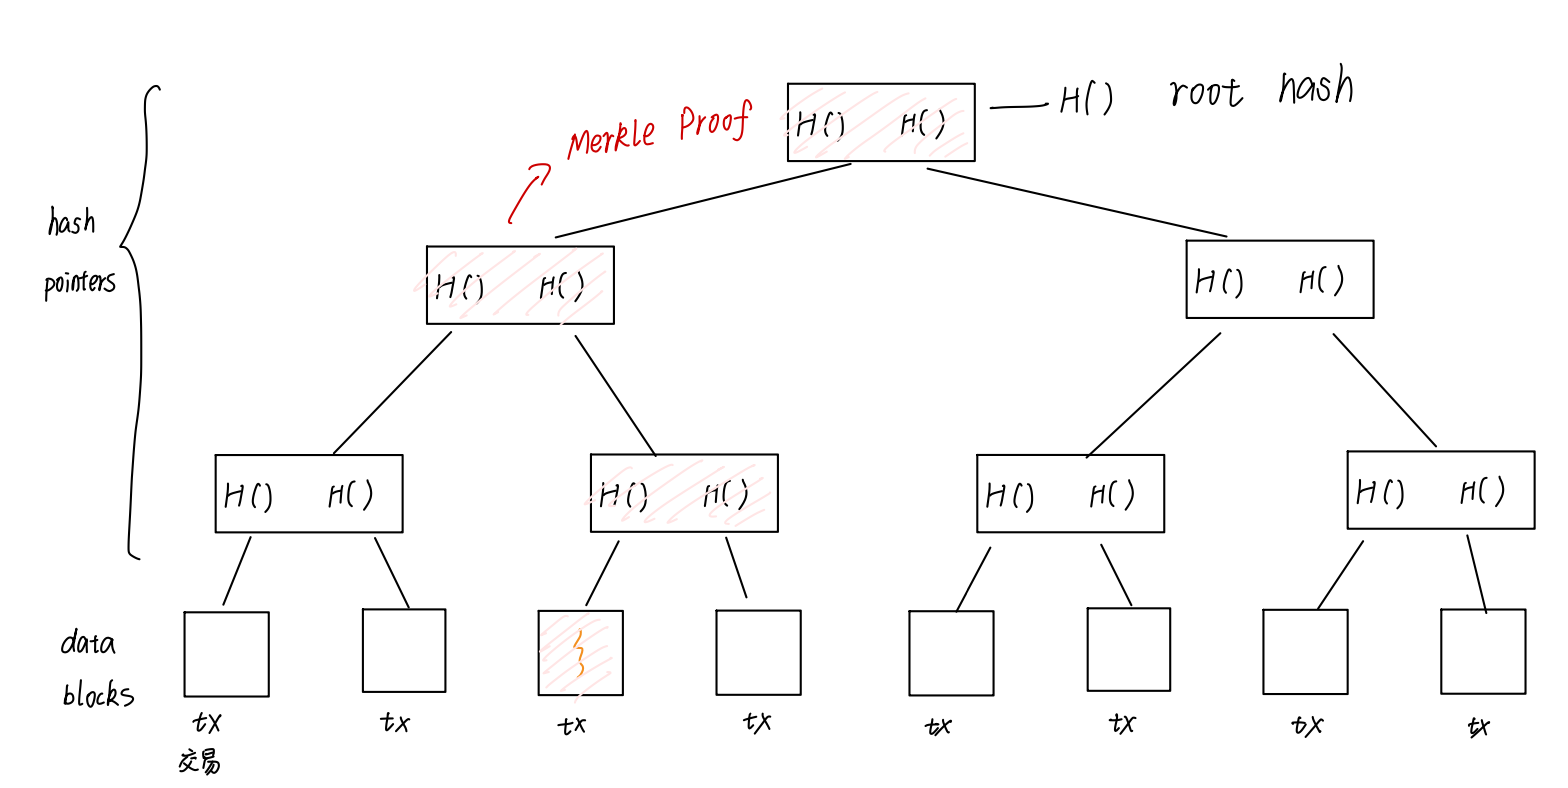
\includegraphics[width=1\textwidth]{./lecture3/img3.png} 
\end{figure}
\begin{itemize}
    \item block header (有root hash)
    \item block body (有交易列表)
\end{itemize}
Merkle tree的作用是可以提供Merkle proof,证明包含某种交易(\textbf{proof of membership / proof of inclusion}),是$O(\log(n))$的时间复杂度。但是如果证明某个交易不包含在Merkle tree中,如果进行所有叶子节点的遍历,时间复杂度是$O(n)$,这时可以考虑采用sorted Merkle tree,时间复杂度降为$O(\log(n))$。
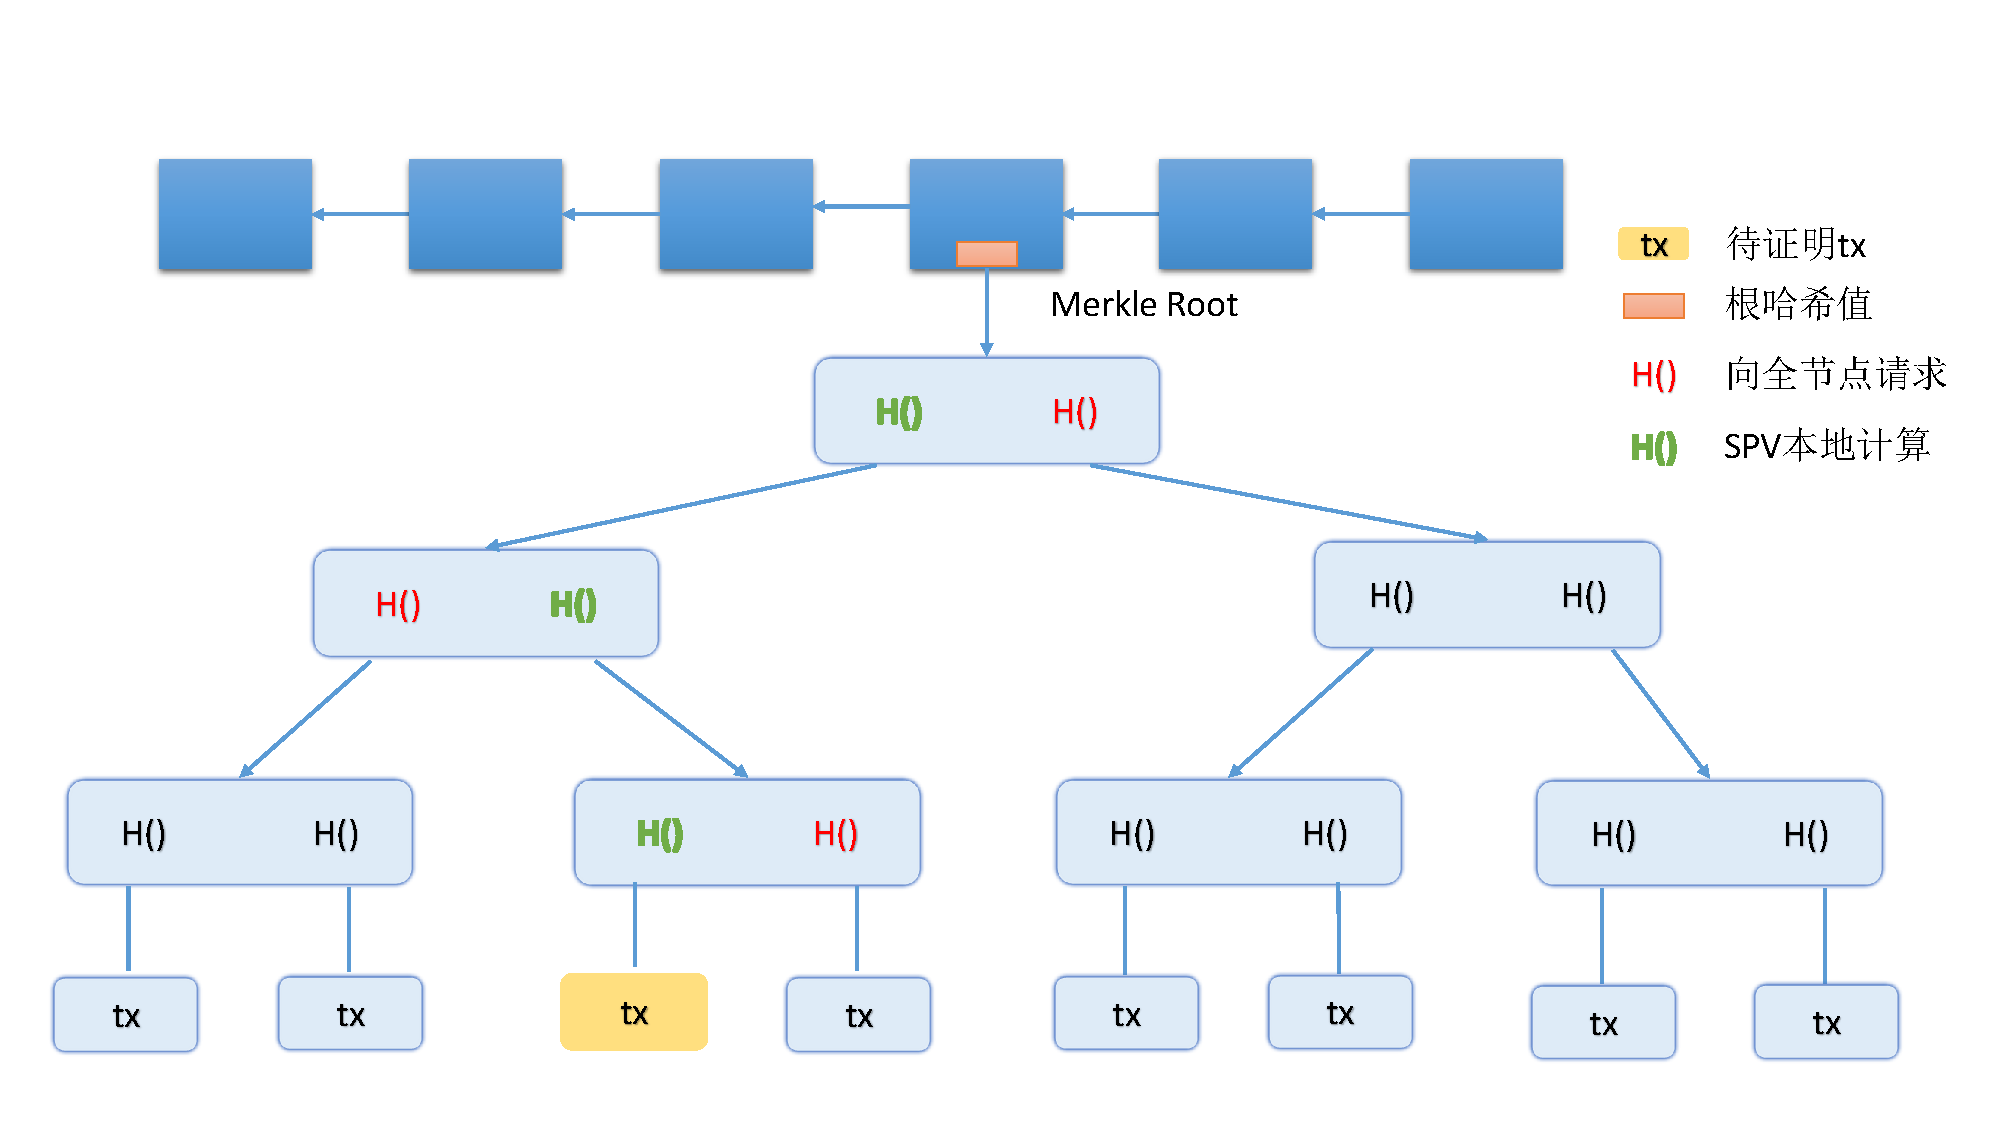
\includepdf[pages=1]{03-BTC.pdf} 
数据结构无环可以用hash pointer。如果有环会出现冲突。
\begin{figure}[H]
    \centering
    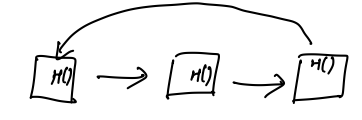
\includegraphics[width=0.5\textwidth]{./lecture3/img4.png} 
\end{figure}
\section{BTC-协议}
如果中央银行要发售电子货币,每张纸币可以由中央银行签名。
\begin{figure}[H]
    \centering
    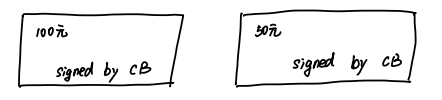
\includegraphics[width=0.5\textwidth]{./lecture4/img1.png} 
\end{figure}
这会出现双花攻击(double spending attack),因为这些电子货币其实就是代码,可以进行复制,我花出去一张100的,我可以复制很多张,继续花费。可以考虑维护一个数据库,给发行的每张货币一个编号,然后记录该货币属于谁,不过这样维护数据库就很麻烦了,而且也并不是去中心化的。
\begin{figure}[H]
    \centering
    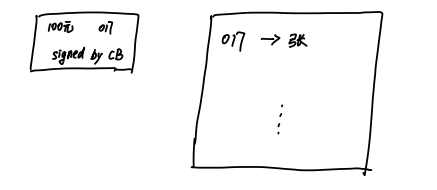
\includegraphics[width=0.5\textwidth]{./lecture4/img2.png} 
\end{figure}
比特币中的交易:
\begin{figure}[H]
    \centering
    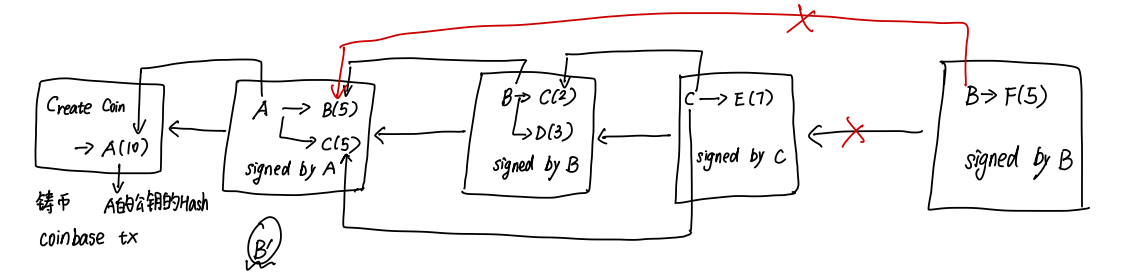
\includegraphics[width=1\textwidth]{./lecture4/img3.png} 
\end{figure}
A要给B转5个比特币,A需要知道B的地址。B也需要知道A的公钥,为了验证A的签名。在上图中,在交易时不仅要说明转账的地址,也要说明币的来源。在图中第二个区块中
\begin{itemize}
    \item 输入:币的来源、A的公钥
    \item 输出:B的公钥的哈希
\end{itemize}
这里就能避免双花,例如图中最后B想给F转5个比特币,可以看到B的5个比特已经花出去了,经过检查是不能再使用的。

脚本验证(Bitcoin Script):将输入与前一个输出拼接在一起,看是否能正确运行。
\begin{figure}[H]
    \centering
    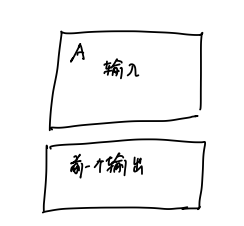
\includegraphics[width=0.3\textwidth]{./lecture4/img4.png} 
\end{figure}
每个块可以有很多交易,组织成Merkle tree。
\begin{figure}[H]
    \centering
    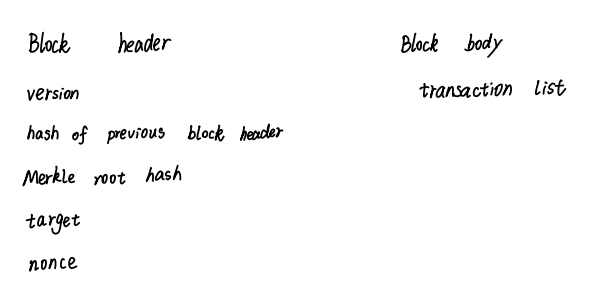
\includegraphics[width=0.7\textwidth]{./lecture4/img5.png} 
\end{figure}
\textbf{挖矿}:H(block header)$\le$target.区块链的另一种画法,因为其实哈希指针计算的是前一个block header中的哈希。
\begin{figure}[H]
    \centering
    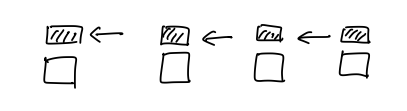
\includegraphics[width=0.6\textwidth]{./lecture4/img6.png} 
\end{figure}
\begin{itemize}
    \item full node: fully validating node,全节点记录所有信息
    \item light node: 轻节点
\end{itemize}

账本的内容要取得分布式的共识(distrubted consensus)。

FLP impossibilty result: 在异步系统中,网络传输时延没有上限,哪怕系统中只有一个成员是faulty,也没法达成共识。

CAP Theorem:任何一个分布式系统,以下3个性质中最多满足2个。
\begin{itemize}
    \item C: Consistency 一致性
    \item A: Availability
    \item P: Partition tolerance
\end{itemize}
Paxos协议满足Consistency性质。
\subsection{Consensus in BitCoin}
重要的问题是:成员(membership)中谁拥有投票权。联盟链(hyperledger fabric)是只有加入链的成员有投票权。

女巫攻击(sybil attack):攻击方产生超过一半的用户。

如果节点能解决puzzle问题,可以获得记账权,有权利发布下一个节点。
\begin{figure}[H]
    \centering
    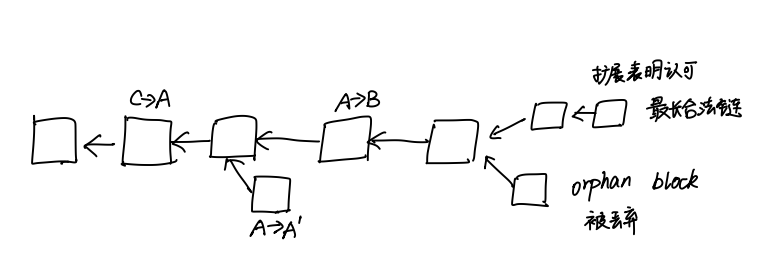
\includegraphics[width=1\textwidth]{./lecture4/img7.png} 
\end{figure}
longest vaild chain: 最长合法链

forking attack: 分叉攻击

block reward: 出块奖励

mining: 挖矿

miner: 矿工

coinbase transaction 是产生币的唯一方法。每隔21万个区块,区块奖励减半,50BTC$\rightarrow$25BTC$\rightarrow$12.5BTC.
\section{BTC-实现}
比特币是基于交易记录的模式(\textbf{transaction-based ledger})。

\textbf{UTXO}: Unspent Transaction Output 还未花掉的交易的输出,为了检测双花,包含产生交易的哈希值以及在交易中的第几个。
\begin{figure}[H]
    \centering
    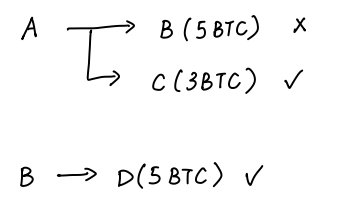
\includegraphics[width=0.4\textwidth]{./lecture5/img1.png} 
\end{figure}
B的5BTC已经花出去了,因此不在UTXO中。

total inputs = total outputs 所有输入=所有输出,但有时候不完全相等,例如所有输入为1BTC,所有输出为0.99BTC,这其中的差值是交易费(transaction fee)。比特币中大约每4年区块奖励会减半,因此到后期的奖励可能大部分来自于交易费。
$$
\frac{\text{21万区块}\times\text{10分钟}}{\text{60分钟}\times\text{24小时}\times\text{365天}} \approx \text{4年}
$$
还有一种模式是基于账户的模式(\textbf{account-based ledger}),例如以太坊。
\begin{figure}[H]
    \centering
    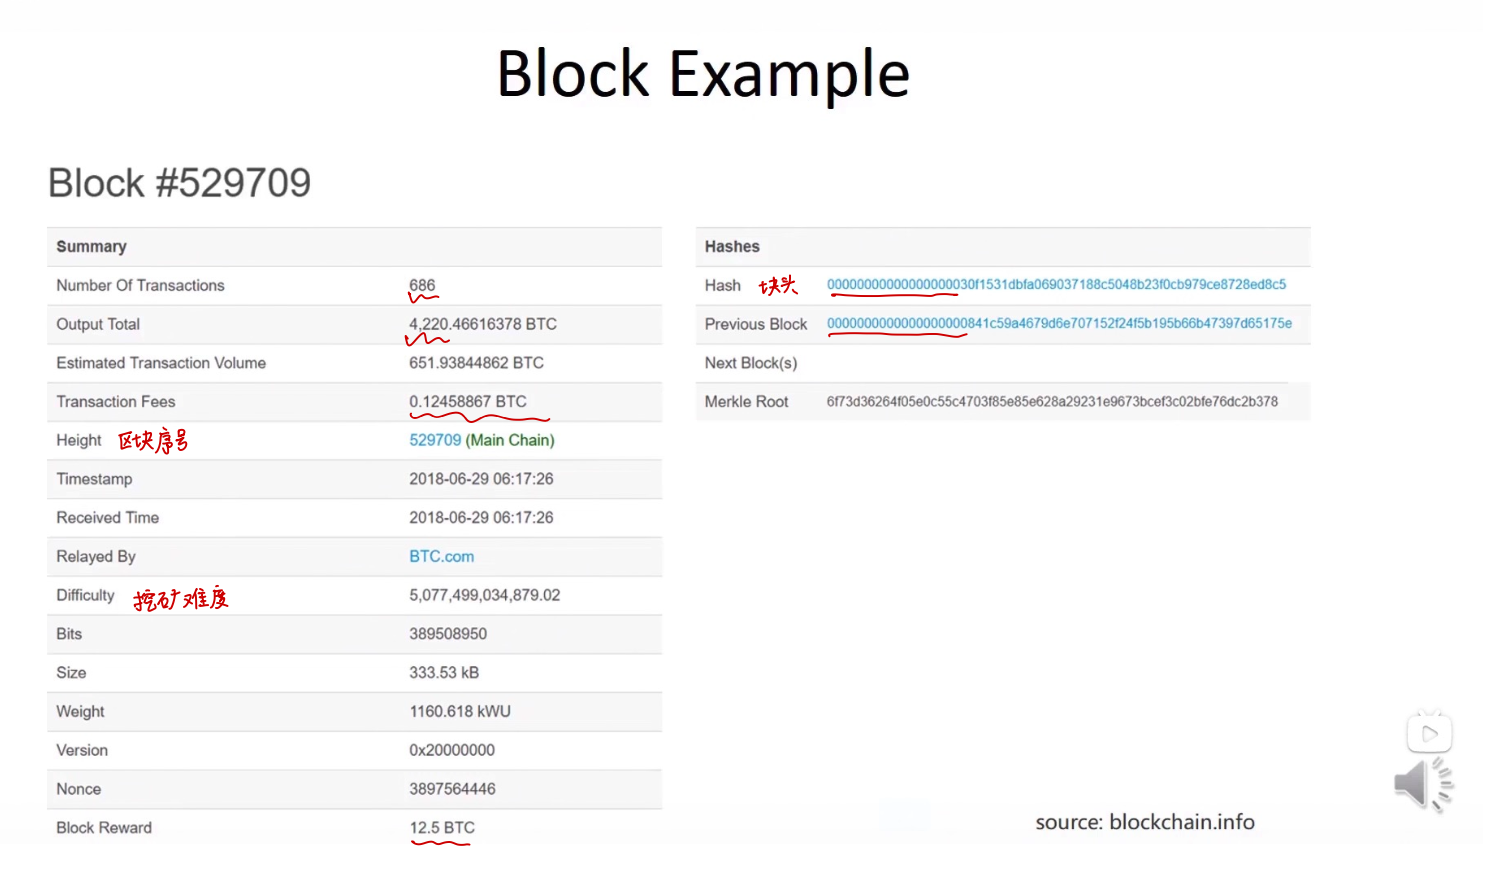
\includegraphics[width=1\textwidth]{./lecture5/img2.png} 
\end{figure}
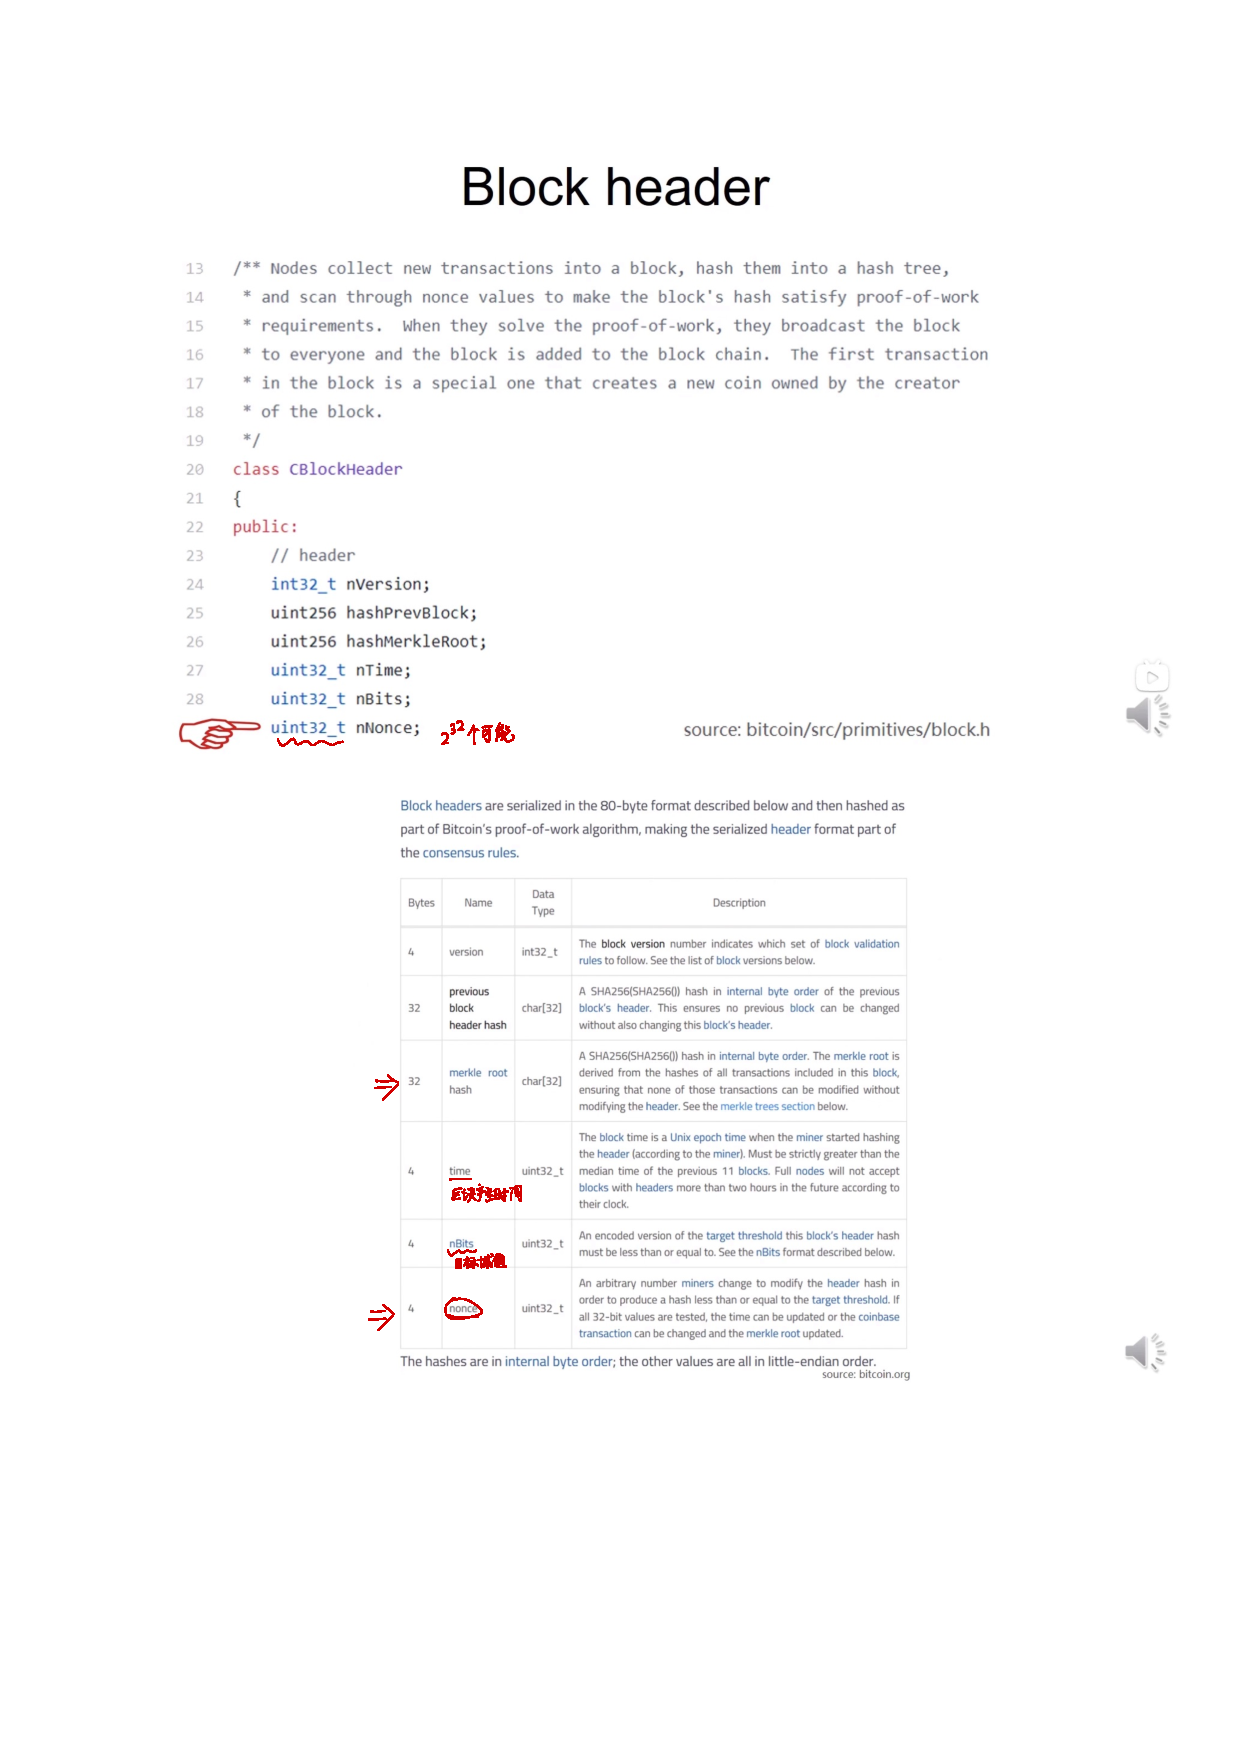
\includepdf[pages=-]{./lecture5/1.pdf} 
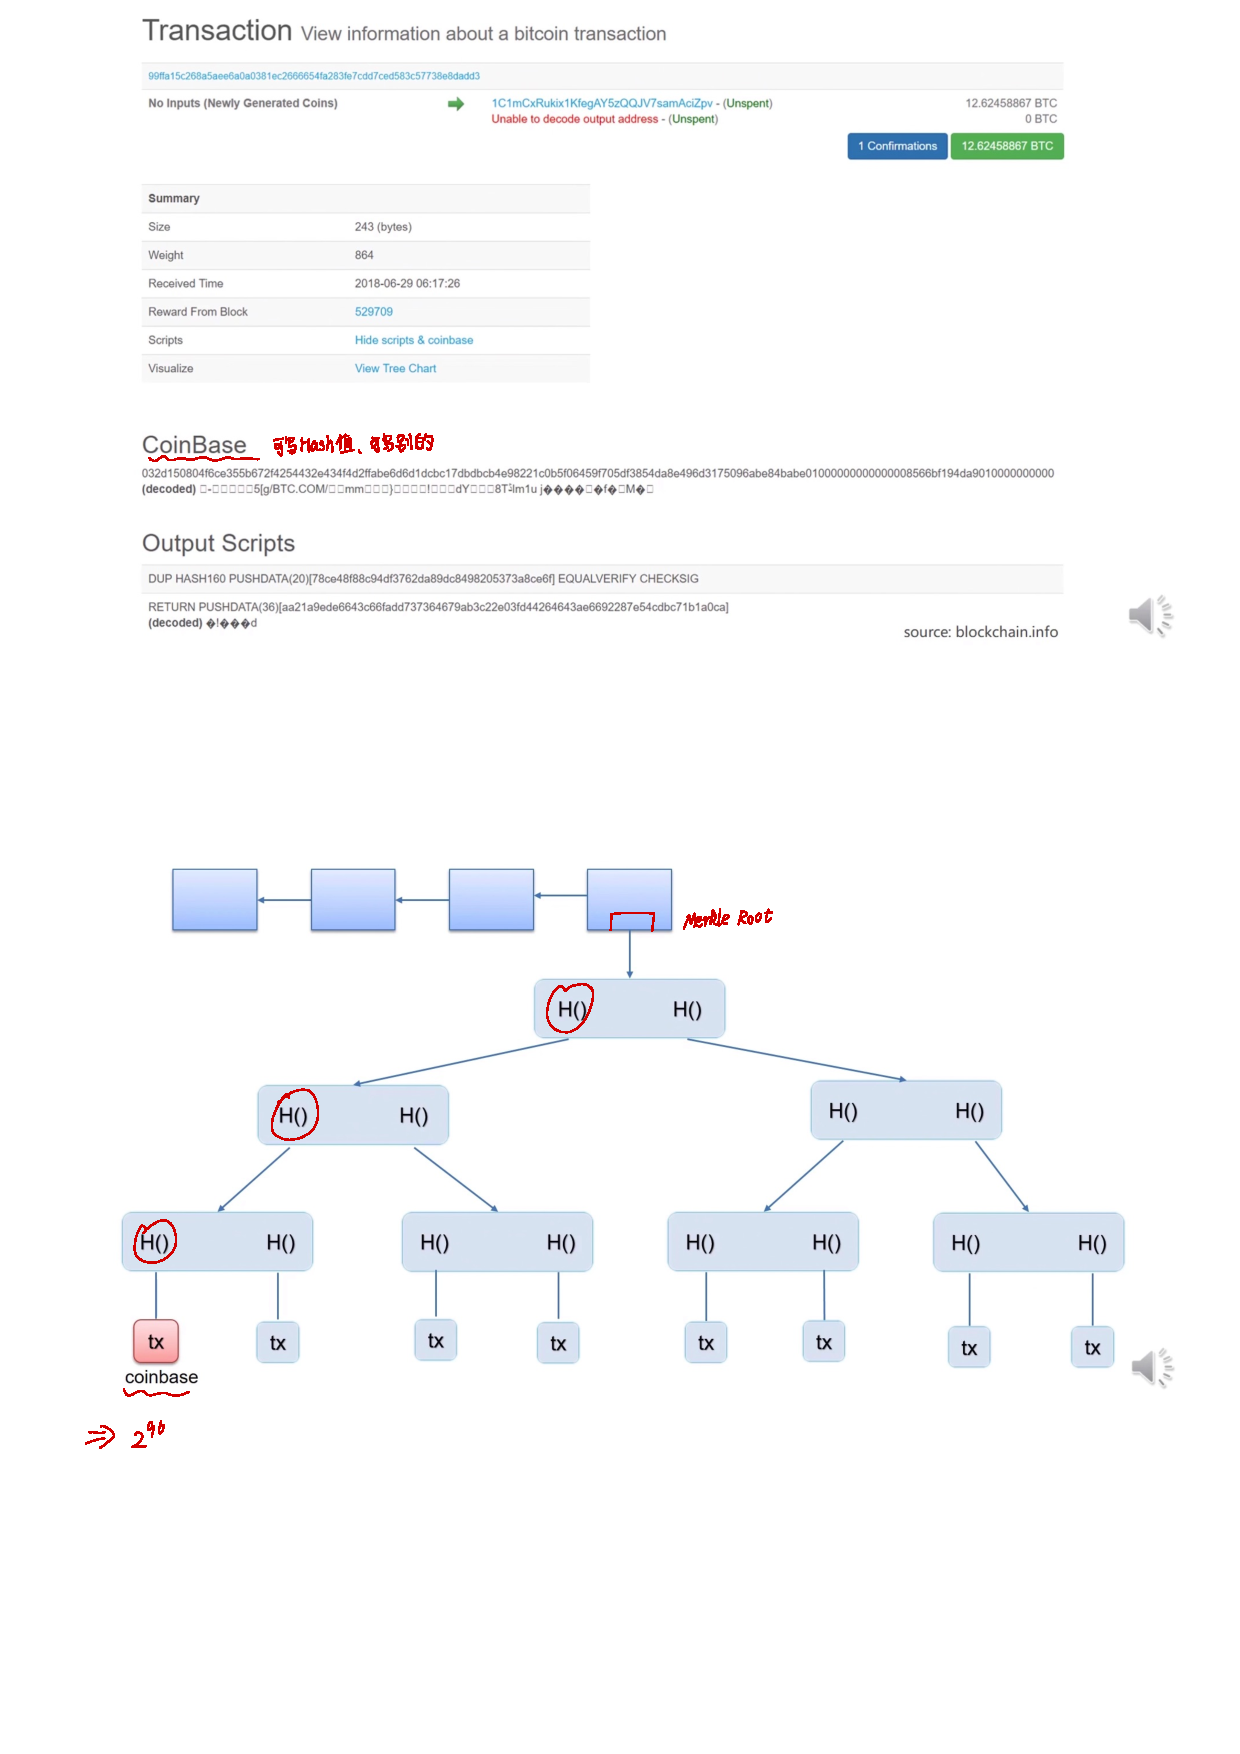
\includepdf[pages=-]{./lecture5/2.pdf} 
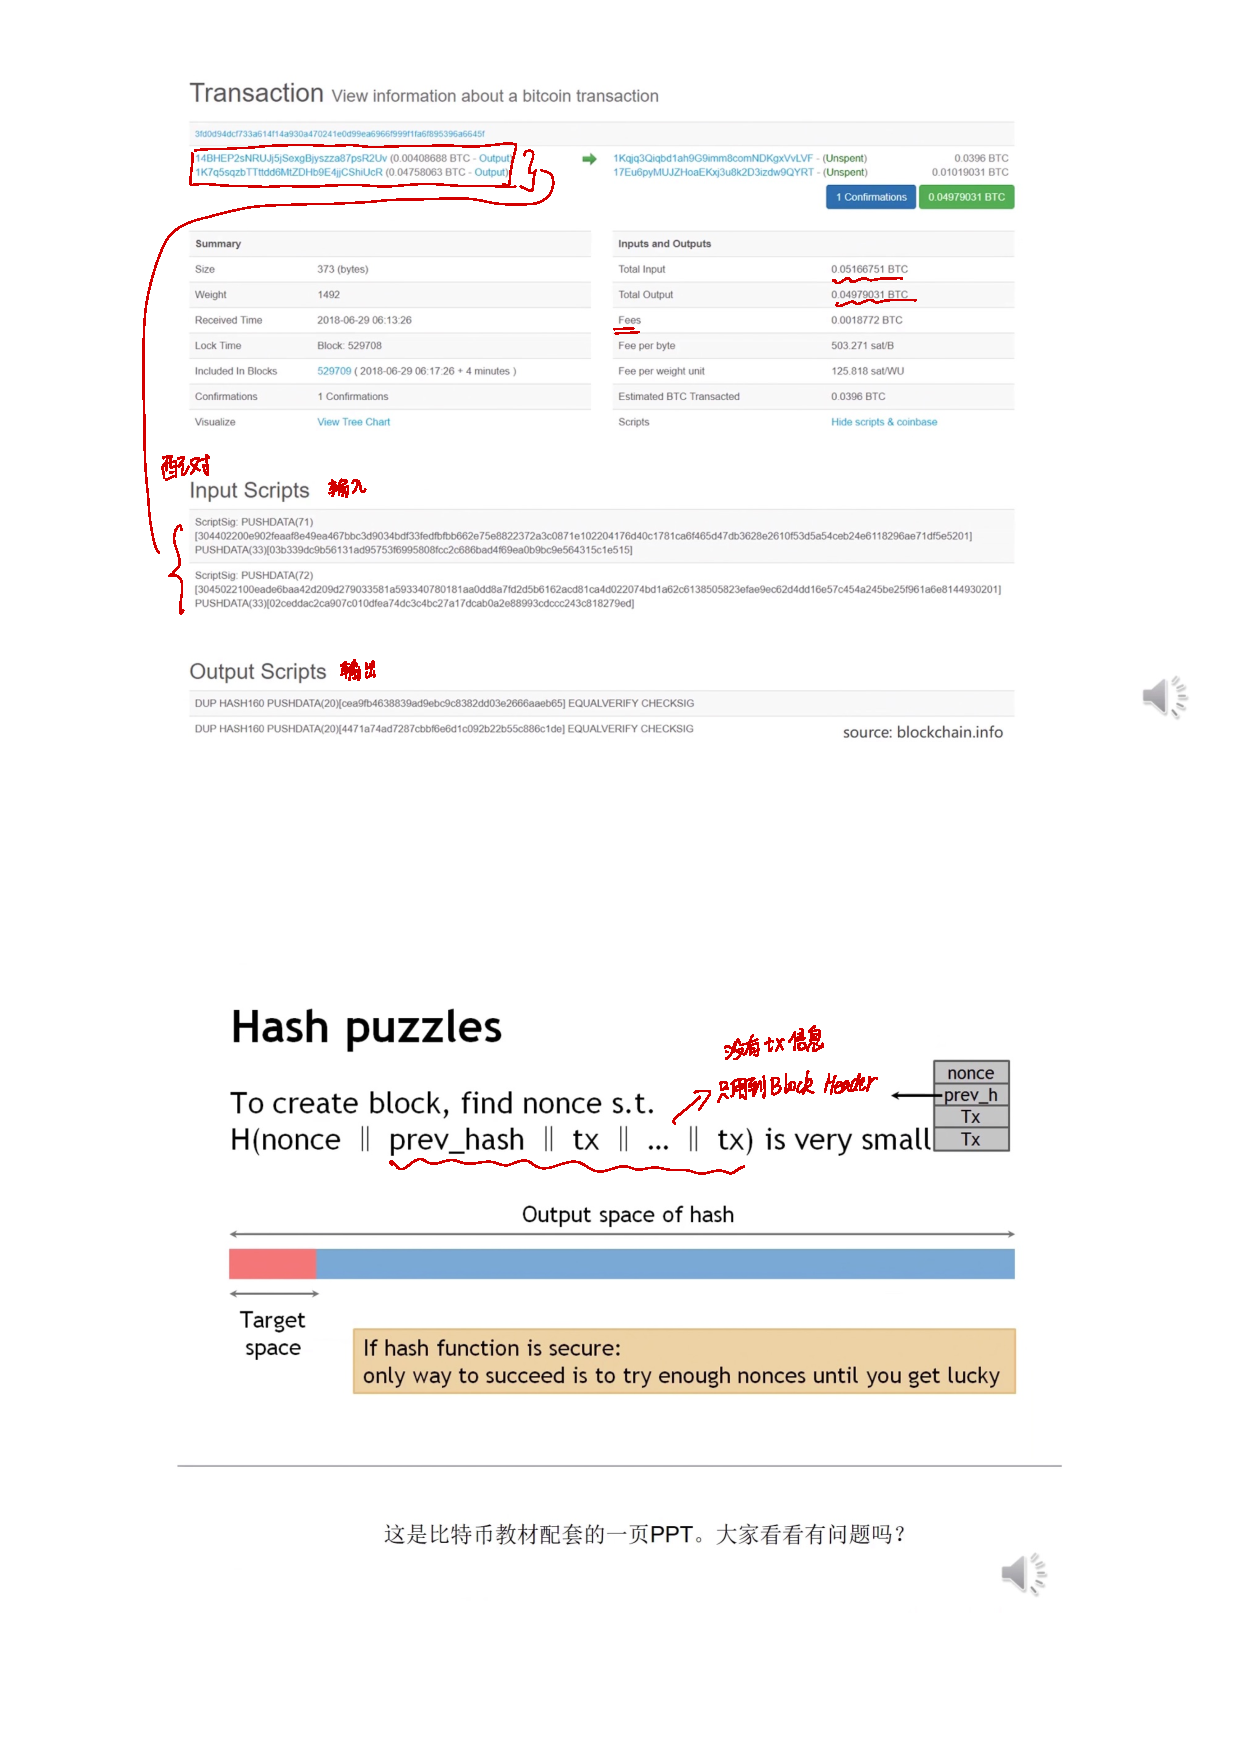
\includepdf[pages=-]{./lecture5/3.pdf} 
每次挖矿尝试看作是\textbf{Bernoulli trial}: a random experiment with binary outcome. Bernoulli process: a sequence of independent Bernoulli trials. Bernoulli process具有无记忆性(\textbf{memoryless})。大量的Bernolli process可用Poisson process近似。

出块时间服从指数分布(exponential distrubtion),也具有无记忆性。
\begin{figure}[H]
    \centering
    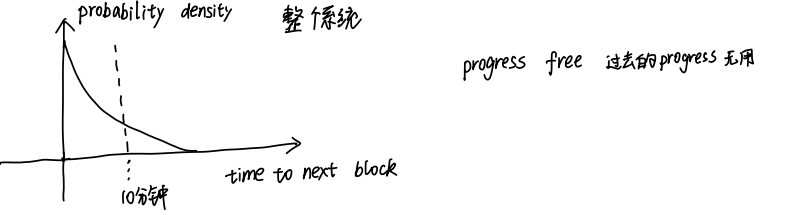
\includegraphics[width=1\textwidth]{./lecture5/img3.png} 
\end{figure}
产生比特币数量构成几何序列(geometric series)
\begin{figure}[H]
    \centering
    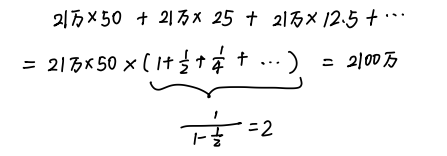
\includegraphics[width=0.5\textwidth]{./lecture5/img4.png} 
\end{figure}
BitCoin is secured by mining.
\begin{figure}[H]
    \centering
    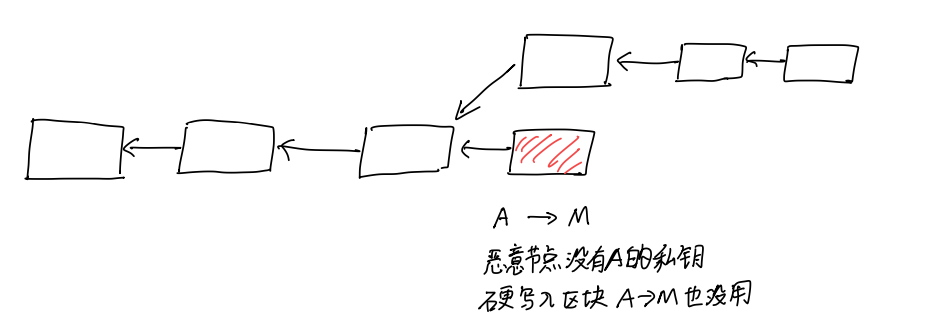
\includegraphics[width=1\textwidth]{./lecture5/img5.png} 
\end{figure}
double spending
\begin{figure}[H]
    \centering
    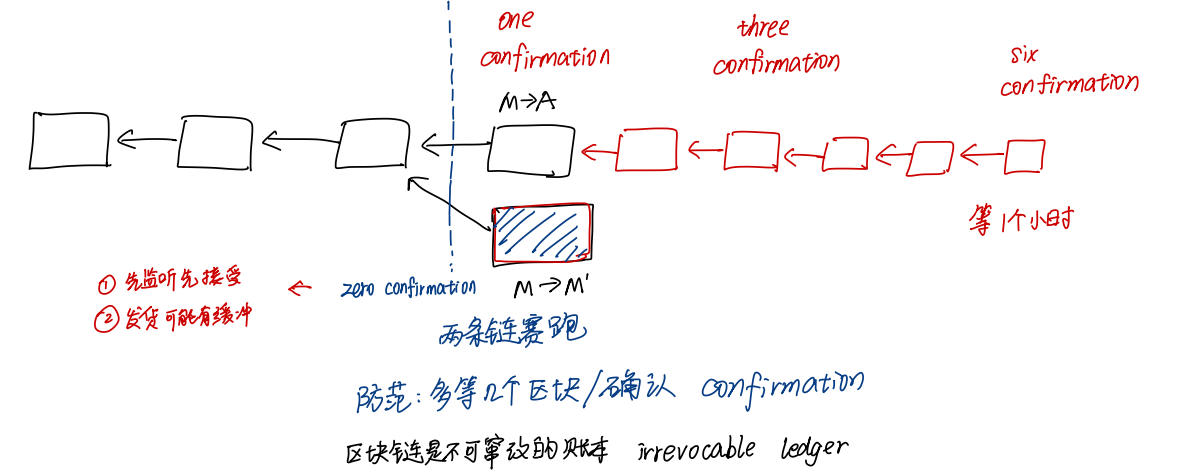
\includegraphics[width=1\textwidth]{./lecture5/img6.png} 
\end{figure}
selfish mining的分叉攻击,挖一长串,然后一下发布,这么做是有风险的。
\begin{figure}[H]
    \centering
    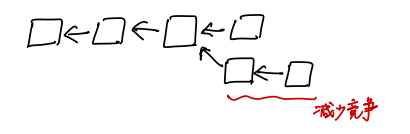
\includegraphics[width=0.5\textwidth]{./lecture5/img7.png} 
\end{figure}
\section{BTC-网络}
上层是application layer: BitCoin Block chain.下层是network layer: P2P Overlay Network.比特币中各节点是对等的。

比特币网络设计原则:simple, robust(鲁棒), but not efficient.

flooding, 邻居节点的选取是随机的,因此两个节点可能地理上相隔很远,网络传输慢,并不是非常有效。全节点维护一个等待上链的集合,第一次听到转发,会在该集合中删除该交易,后续不转发。区块大小限制在1M。网络传播是尽力交付(best effort)。

\section{BTC-挖矿难度}
H(block header) $\le$ target,挖矿难度
$$
\text{difficulty} = \frac{\text{difficulty\_1\_target}}{\text{target}}
$$
难度1,target更大。挖矿难度与target成反比。
\begin{figure}[H]
    \centering
    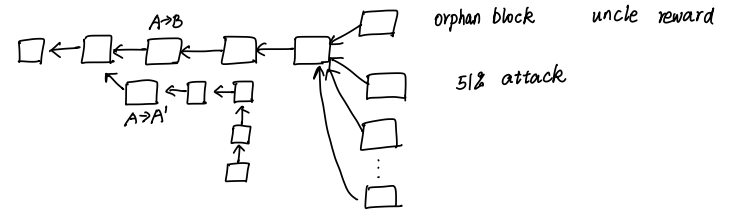
\includegraphics[width=1\textwidth]{./lecture7/img1.png} 
\end{figure}
出块时间越短,出现分叉的可能更多。

以太坊协议 ghost,平均出块时间需要保持稳定。

调整挖矿难度:
$$
\text{target} = \text{target} \times \frac{\text{actual time}}{\text{expected time}}
$$
其中,acutual time是最近挖出2016区块的时间,期望时间expected time = $2016 \times 10$,理想的挖出2016个区块的时间是两周。难度最大增长4倍,最小也是缩小4倍。
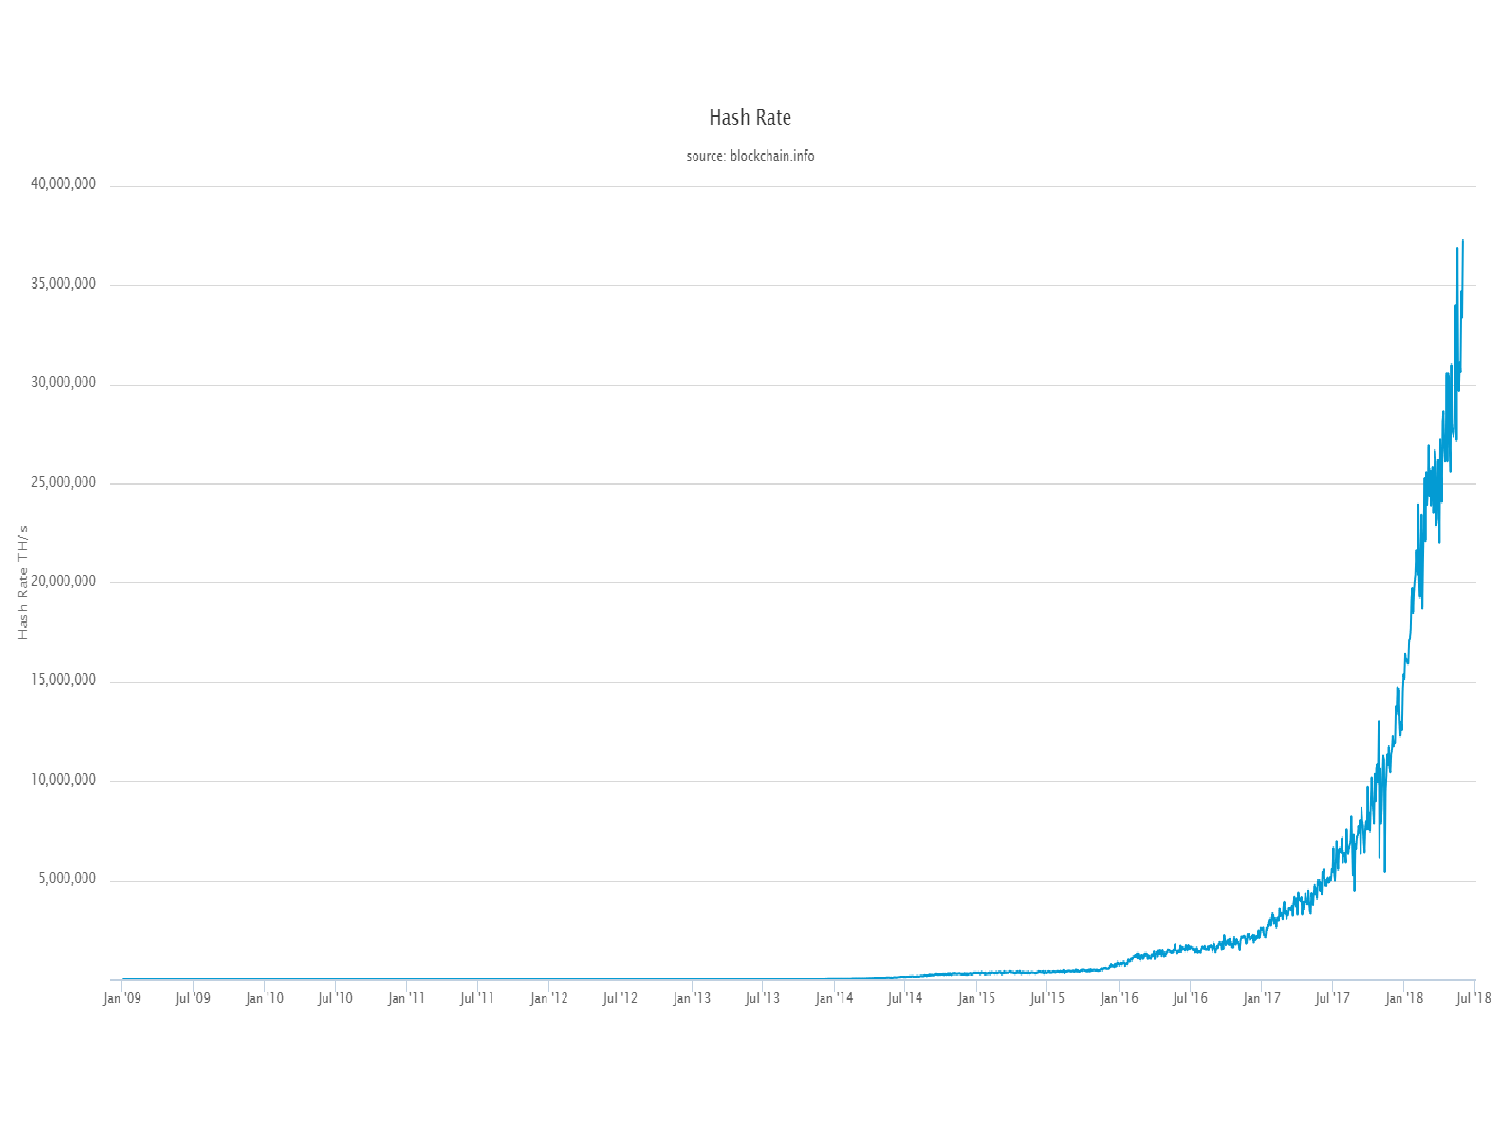
\includepdf[pages=-,nup=1x2]{07-BTC.pdf} 
\section{BTC-挖矿}
全节点验证合法性包括:每个交易合法、发布区块难度以及延伸最长合法链。

挖矿无记忆性,memoryless以及progress free。

比特币安全性由密码学安全与共识机制保证,这个前提是大部分节点是好的节点。

CPU$\rightarrow$ GPU挖矿$\rightarrow$ ASIC(Application Specific Integrated Circuit)芯片,ASIC芯片只能挖同一个mining puzzle的货币。有的币设计之初选择Alternative mining puzzle,设计出发点是ASIC resistance。

矿池,一个矿主(pool manager)下面有许多矿工(miner),矿主承担全节点其他功能。矿池的出现解决矿工收入不稳定的问题。通过工作量证明来分配收入,例如本来要求nonce使得前面60个为0,降低难度,如果求出该问题的nonce,则获得一个share,将almost vaild block提交给矿主,证明工作,最后根据提交的share数量分配奖励。

转换矿池很容易,大型矿池如果有51\%算力,可发起攻击:
\begin{itemize}
    \item 分叉攻击
    \begin{figure}[H]
        \centering
        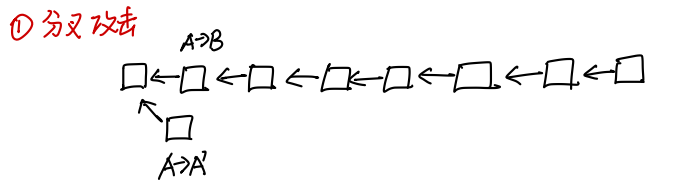
\includegraphics[width=0.7\textwidth]{./lecture8/img1.png} 
    \end{figure}
    \item Boycott 封锁,和A有关交易都不包含,马上分叉
    \begin{figure}[H]
        \centering
        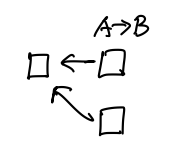
\includegraphics[width=0.2\textwidth]{./lecture8/img2.png} 
    \end{figure}
\end{itemize}
但是拥有51\%以上算力不能盗币,因为没有别人账户的私钥。如果强行发布不合法的区块,会造成分叉。

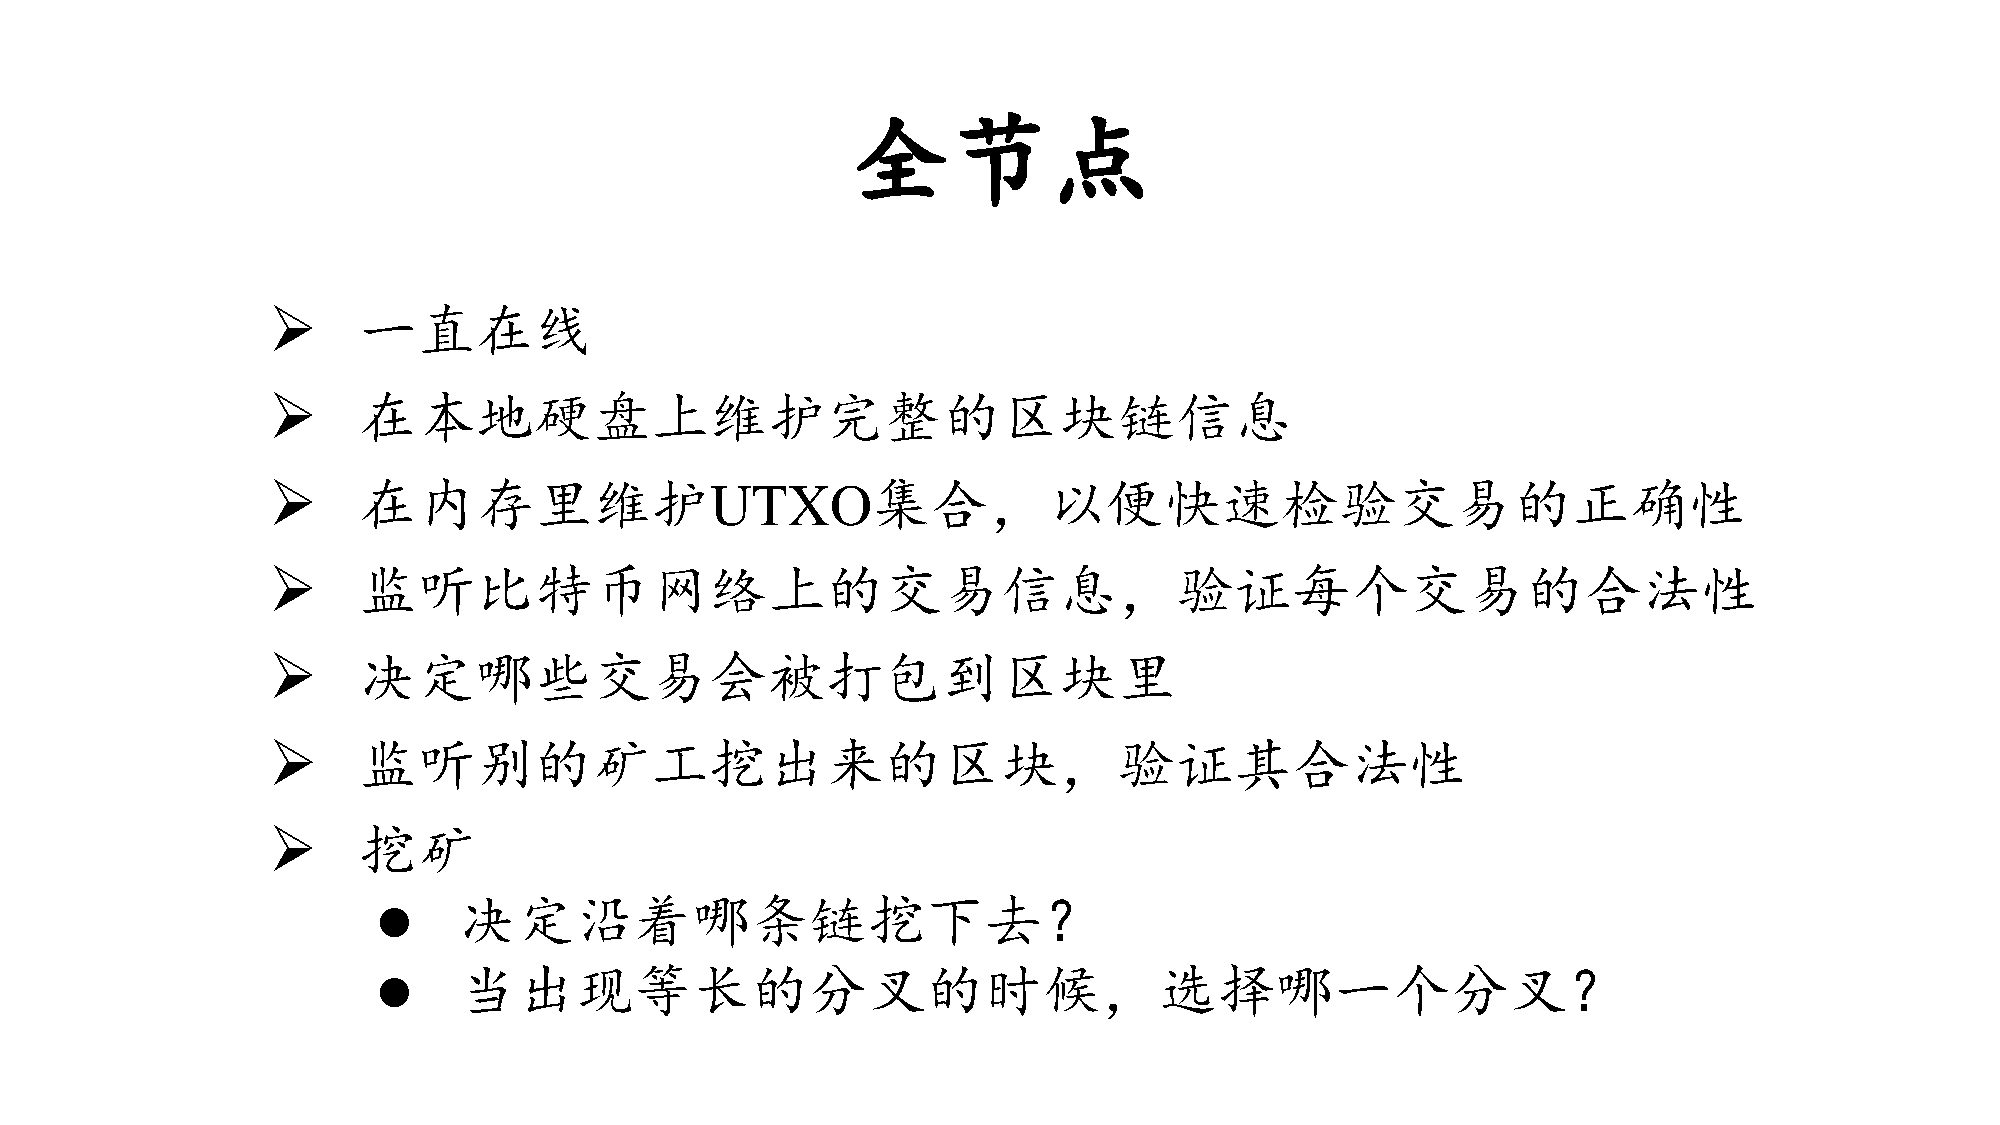
\includepdf[pages=-,nup=1x2]{08-BTC.pdf}  
\section{BTC-比特币脚本}
交易结构:
\begin{itemize}
    \item version: 比特币协议版本号
    \item locktime: 生效时间
    \item blockhash: 交易所在区块的hash值
    \item blocktime: 区块产生时间
\end{itemize}
交易的输入:
\begin{itemize}
    \item "txid"与"vout",表示币的来源
    \item "scriptSig"表示输入脚本
\end{itemize}
交易的输出:
\begin{itemize}
    \item "value":输出金额
    \item "n":序号
    \item "scriptPubKey": 输出脚本
    \item "reqSigs":需要多少个签名
    \item "type": 输出类型
\end{itemize}
redeemScript: 赎回脚本

多重签名:
\begin{itemize}
    \item 多重签名要求N个人中有M个签名
    \item x是代码实现的bug,往栈里多压入一个元素
    \item 输入脚本中M个签名的顺序要与输出脚本中的pubkey相同
\end{itemize}

用P2SH实现多重签名的好处是在用户端,也就是输出脚本处,只需要得知赎回脚本的哈希值即可,不需要N个公钥。同时赎回脚本中方便修改N与M的值。

Proof of Burn
\begin{itemize}
    \item RETURN: 无条件返回错误,可用于证明销毁比特币
    \item 可以往区块链中写入内容,digital commitment,比如用作知识产权。还有另一个域coinbase域,可以往区块链中写入内容。
\end{itemize}

在实际中,操作中含有前缀,例如OP\_CHECKSIG、OP\_DUP,课程中做了简化。

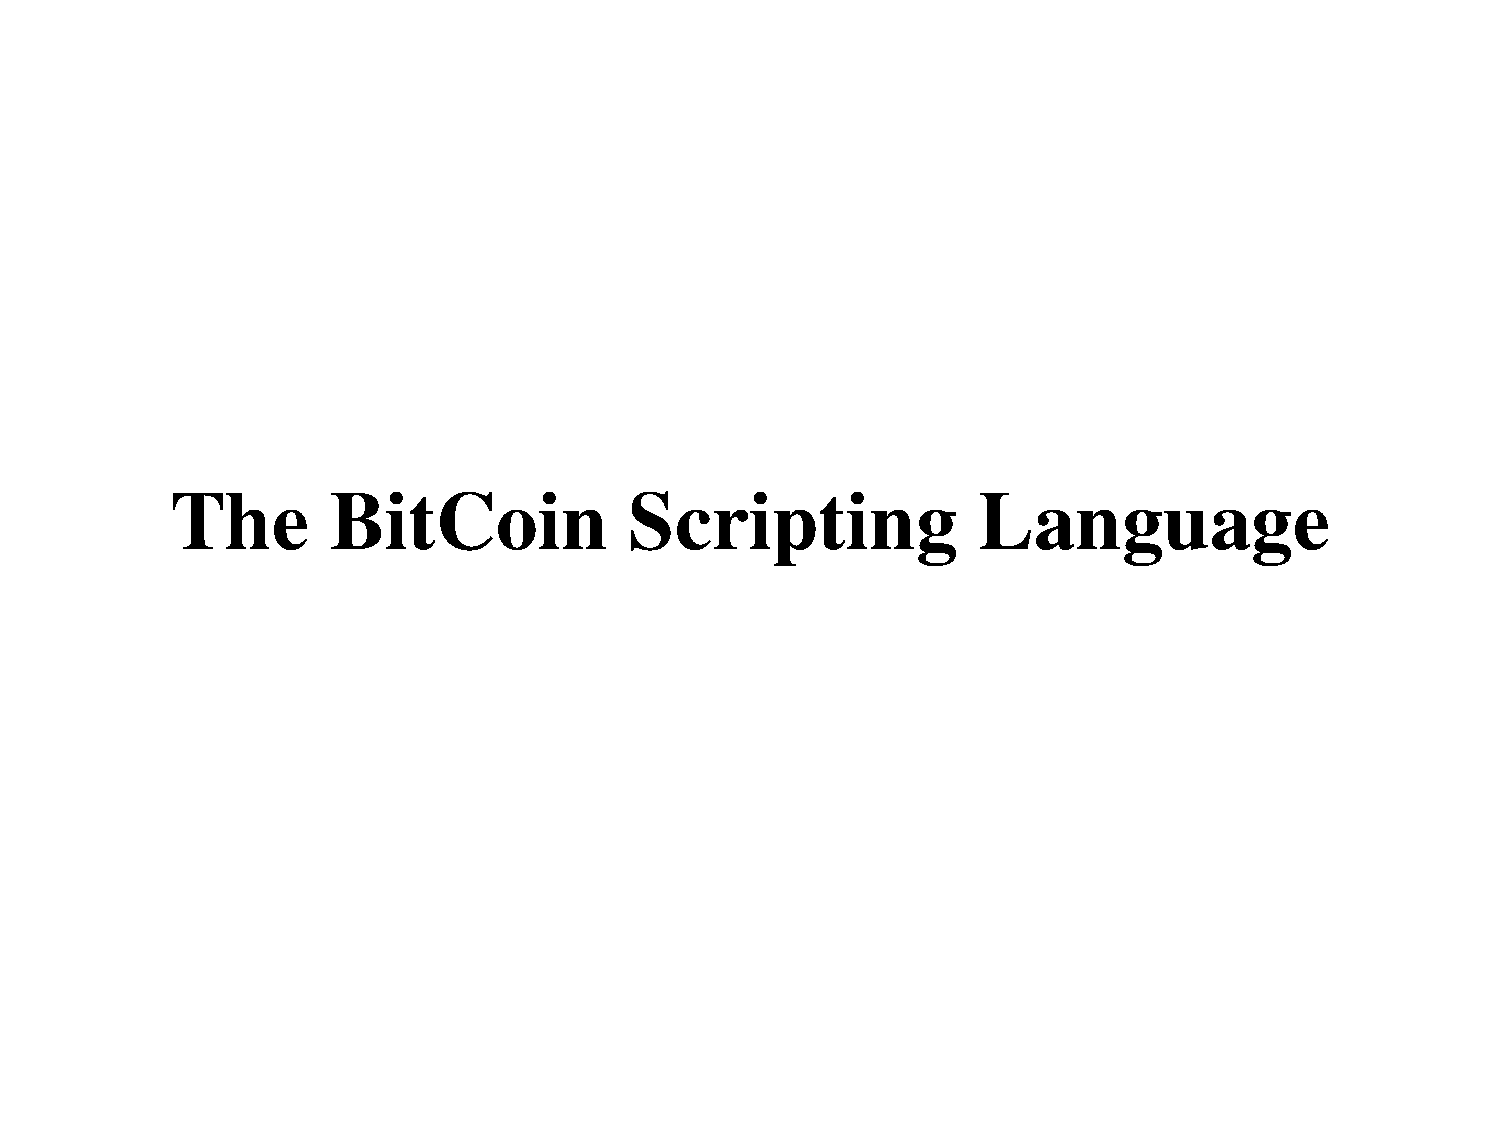
\includepdf[pages=-,nup=1x2]{09-BTC.pdf}  
\section{BTC-分叉}
\begin{itemize}
    \item state fork:当前状态产生分歧,例如分叉攻击(forking attack),也叫做deliberate fork。
    \item protocol fork:对协议产生分歧
\end{itemize}
还有一种分类是分为硬分叉和软分叉。
\subsection{hard fork}
例如block size limit的改变,原来为1M,当block size limit为1M时,一个交易大约是250个字节,一个block可以产生1000,000/250 = 4000个交易,而一个block产生需要10分钟,因此每秒产生4000/(60 $\times$ 10) $\approx $7个交易。这个交易产生的数量太少,并且会有延迟,一个交易可能这个区块没写进去,会等到下一个区块,这就要等待10分钟。考虑block size limit从1M $\rightarrow$ 4M。
\begin{figure}[H]
    \centering
    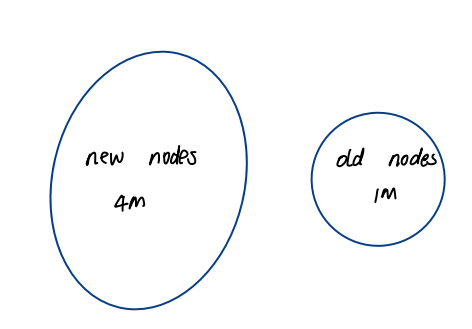
\includegraphics[width=0.6\textwidth]{./lecture10/img1.png} 
\end{figure}
如上图所示,拥有大多数算力节点承认区块大小限制为4M,旧节点承认区块大小为1M。
\begin{figure}[H]
    \centering
    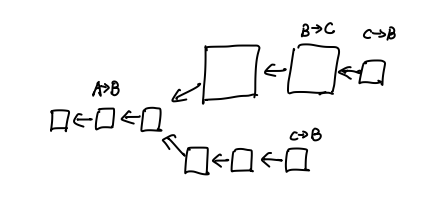
\includegraphics[width=0.6\textwidth]{./lecture10/img2.png} 
\end{figure}
这样会造成永久性分叉,旧节点不承认新节点,会按照原来的链挖,而新节点也是承认1M区块大小的。如果出现下面的链进行交易回放,如C$\rightarrow$B,可以加上chainID来解决这个问题。
\subsection{soft fork}
比特币协议中加一些限制,使得原来合法的交易变得不合法,造成了软分叉。例如区块的大小限制1M变为0.5M。
\begin{figure}[H]
    \centering
    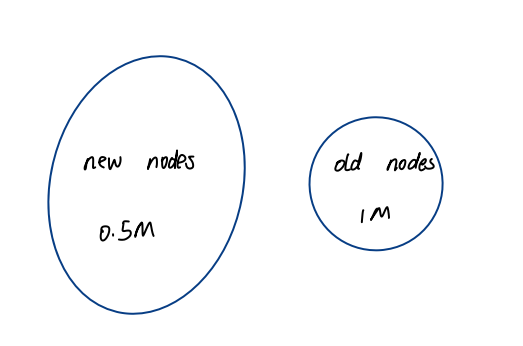
\includegraphics[width=0.6\textwidth]{./lecture10/img3.png} 
\end{figure}
软分叉是临时的,旧节点也认可新节点的链,旧节点会在最长合法链后面挖,不然自己就白挖了。
\begin{figure}[H]
    \centering
    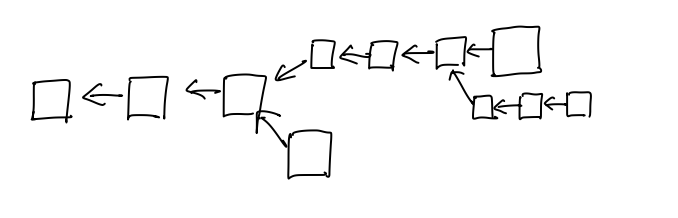
\includegraphics[width=0.6\textwidth]{./lecture10/img4.png} 
\end{figure}
现实中的软分叉:给目前域赋予新的含义,例如coinbase域。原来调整extra nonce,有4bytes,搜索空间是$2^{32}$,可以加上coinbase的前8bytes,搜索空间变为$2^{96}$。

我们知道Merkle proof可以证明某个交易是否在区块里,但是如果想证明某个账户A上有多少钱,全节点可以查看账户A在UTXO对应的输出,对于区块链钱包,也就是轻节点,可以向全节点发出一个请求,全节点返回一个结果,但无法证明该结果是否正确。解决方法是将UTXO组织成一个Merkle tree, 算出根哈希值,放在coinbase里,coinbase里的内容会放在block header里,因此也会改变Merkle tree的根哈希值,当做Merkle proof时,也就验证了结果是否正确。

比特币中著名软分叉例子:P2SH(Pay to Script Hash),支付给一个赎回脚本(redeem Script)的哈希。
\subsection{小结}
\textbf{hard fork}:只有所有节点都更新软件,系统中才不会出现永久性分叉。

\textbf{soft fork}:只要系统中拥有半数以上算力的节点更新了软件,系统中就不会有永久性分叉。

\section{BTC-问答}
\begin{itemize}
    \item 转账交易的时候,如果接收者不在线怎么办?
        
    不需要接收者在线。
    \item 全节点收到一个交易,有没有可能这个交易的接收地址是以前从来没有听说过的。
    
    可能。比特币账户创建本地产生公私钥对。
    \item 如果账户的私钥丢失了该怎么办?
    
    私钥丢失没办法,账户上的钱变成死钱,没办法取出来。

    注:交易所一般要经过身份验证,私钥实际是交易所保管。加密货币的交易所目前缺少监管。交易所Mt. Gox被黑客攻击。
    \item 如果你的私钥泄漏了怎么办?比如账户上出现了可疑交易。
    
    应该将账户上的钱尽快转到另一个安全的账户上。

    \item 如果转账的时候写错了地址怎么办?
    
    没有办法取消已经发布的交易。

    注:digital commitment,用Proof of Burn,将哈希值放在OP\_RETURN后面。A$\rightarrow$B,有人将转账的哈希值变成digital commitment生成的哈希值。这个做法不提倡,转账交易会永久保存在UTXO中,对全节点不友好。

    \item OP\_RETURN无条件返回错误,怎么写到区块链中?
    
    OP\_RETURN写在当前脚本的输出里,验证当前交易的合法性时,是不会执行OP\_RETURN的。有人想花这笔交易的钱时,才会执行这个交易的输出脚本。

    \item 会不会有的矿工偷答案?你怎么知道是哪个矿工最先找到这个符合要求的nonce?
    
    发布的区块里有coinbase tx,有一个到矿工A的收款地址,如果要偷答案,就要改变收款地址,但是这会改变Merkle tree的根哈希值。而nonce在block header,如果改变,原来找到的nonce就作废了。

    \item 你怎么知道交易费该给哪个矿工?
    
    事先不需要知道哪个矿工得到交易费。只要total inputs > total outputs,差额就是交易费。
\end{itemize}
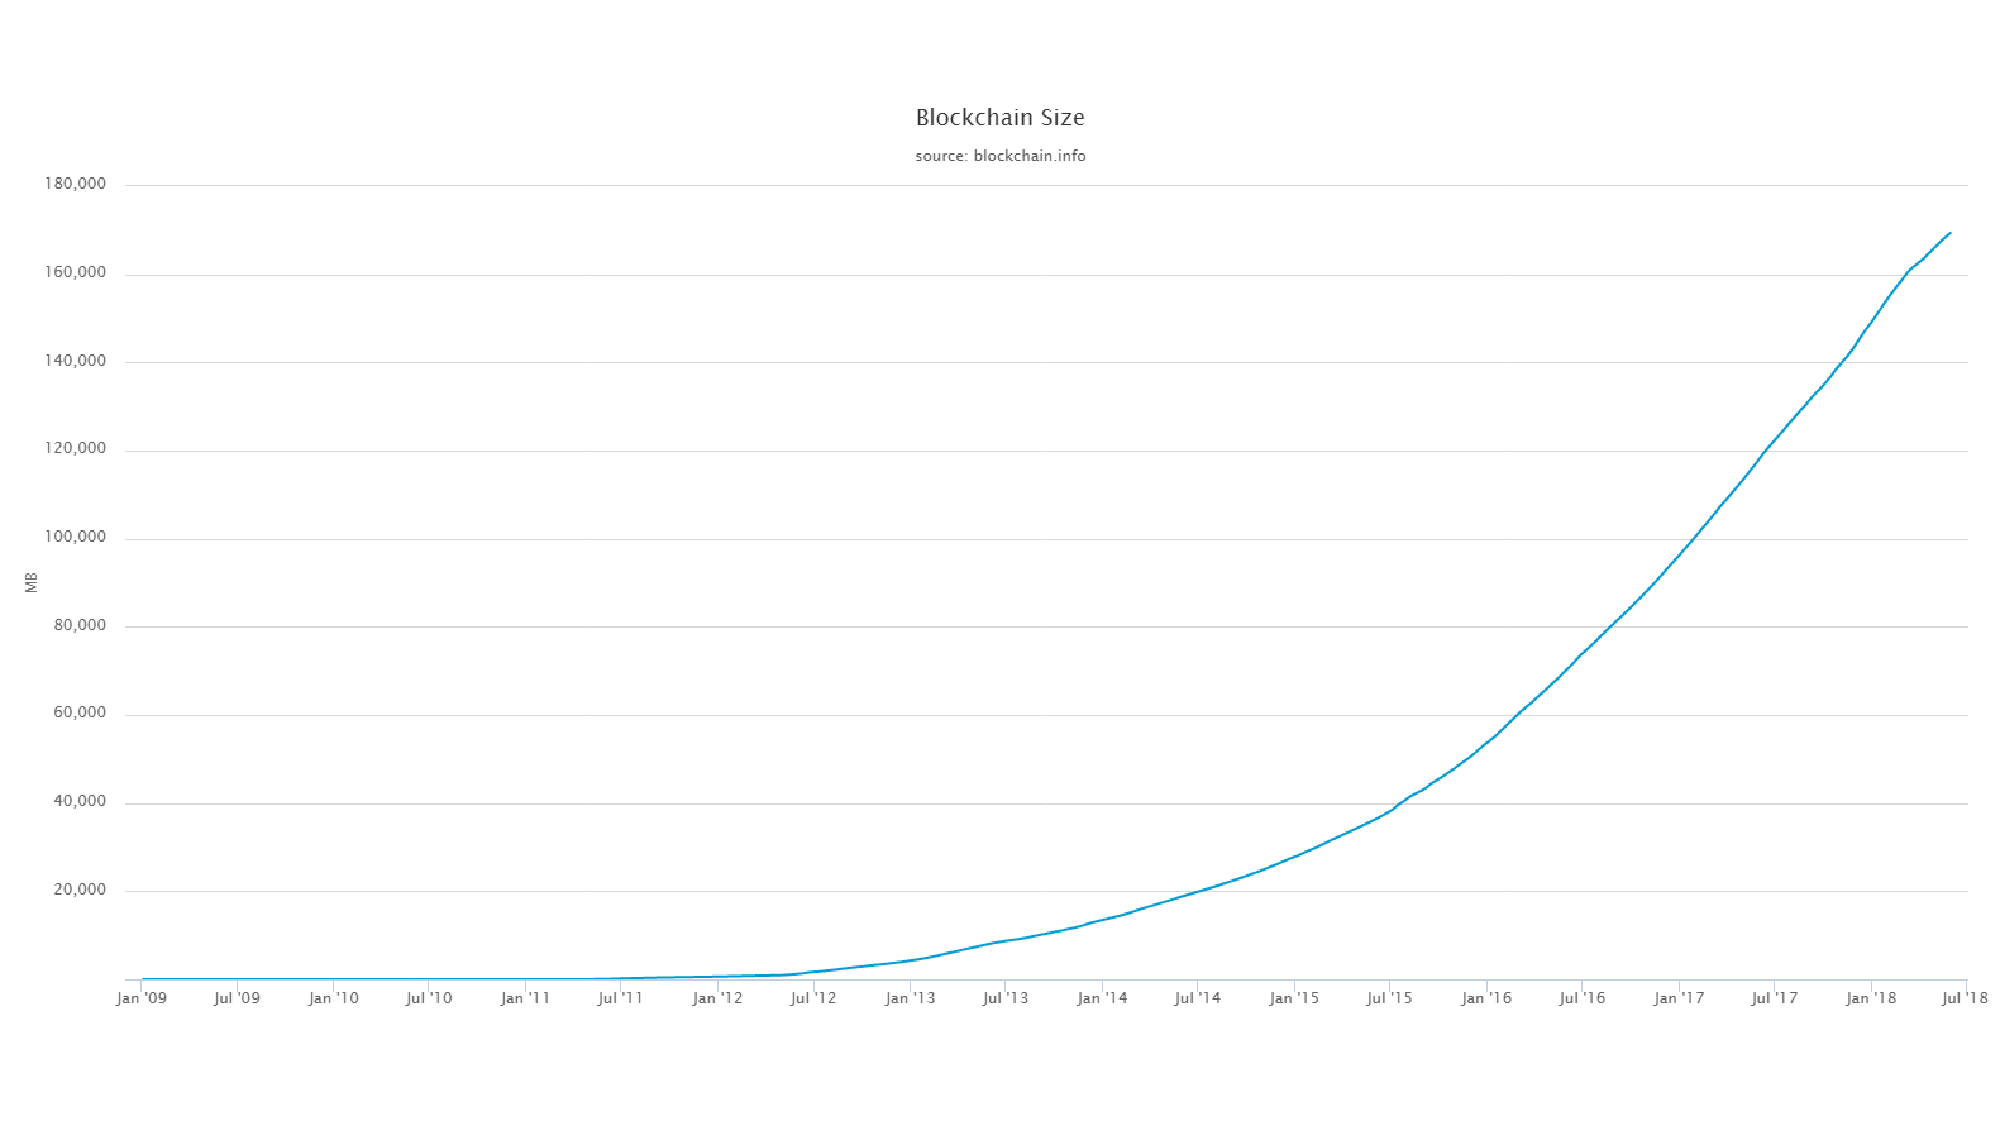
\includepdf[pages=-,nup=1x2]{11-BTC.pdf} 

\section{BTC-匿名性}
\subsection{匿名与隐私}
Bitcoin and anonymity
匿名和隐私(privacy)保护联系在一起。

比特币中用的化名pseudonymity,比特币的匿名不是真的匿名。匿名性没有现金好,但是现金不容易保管和运输。如果银行用化名,匿名性要比比特币好。区块链的账本是完全公开的,银行的账本不是完全公开的。

不同账户之间关联有可能破坏匿名性。网上购物,允许有多个输入和输出。

Inputs: addr1(4BTC), addr2(5BTC)

Outputs: addr3(6BTC), addr4(3BTC)

addr1和adder2很有可能是同一个人的。输出地址一般有一个找零钱的地址。addr4是找零地址,也可以将输入地址和输出地址关联。常用的比特币钱包就几种。找到其中产生地址的规律就可以关联起来。

地址账户和现实世界的身份产生关联。任何比特币货币和实体世界发生联系,就可能泄漏身份。例如资金的转入和转出、用比特币做支付。商家支持比特币支付,延迟大,交易费贵。

信用卡号码取哈希值公开,但是通过几次特定时间消费,进行过滤后可以定位到人。比特币交易记录都是公开的。

中本聪的匿名性保护的最好,没有花费比特币。

网站Silk road,有人管它叫eBay for illegal drugs。卖的是违禁品,支付用比特币,网络层是TOR,美国用匿名邮寄服务。运行两三年就被查封了。第二版Silk road 2。比特币的匿名性没有我们想象中的那么好。

hide your identity for whom?不想向谁暴露身份?如果是向邻居保持匿名,比较容易实现。

采取什么样的方法尽可能提高匿名性?

application layer

--------

network layer

提高匿名性从两个方面入手。网络层的匿名性比较好解决,普遍的是多路径转发,洋葱路由TOR就是这个原理。应用层把各个不同的币混在一起(coin mixing),让人分不清这些币从哪里来的,真正实施起来有些困难。在区块链里目前没有信誉度高的coin mixing服务,因为它们也要匿名,跑路就没办法了。有一些应用带有coin mixing性质,比如在线钱包,但在线钱包并不保证履行这个功能。加密货币的交易所天然的有coin mixing性质,前提是交易所不会泄漏记录。

保护隐私难度大,本质是区块链账本公开且不可篡改。

\subsection{零知识证明}
签名证明知道私钥,但是泄漏了私钥的签名。是不是零知识证明有点争议。

\textbf{同态隐藏}
\begin{itemize}
    \item 加密函数值不会出现碰撞。
    \item 加密函数不可逆。和哈希函数里的hiding property类似。
    \item 同态运算。
\end{itemize}
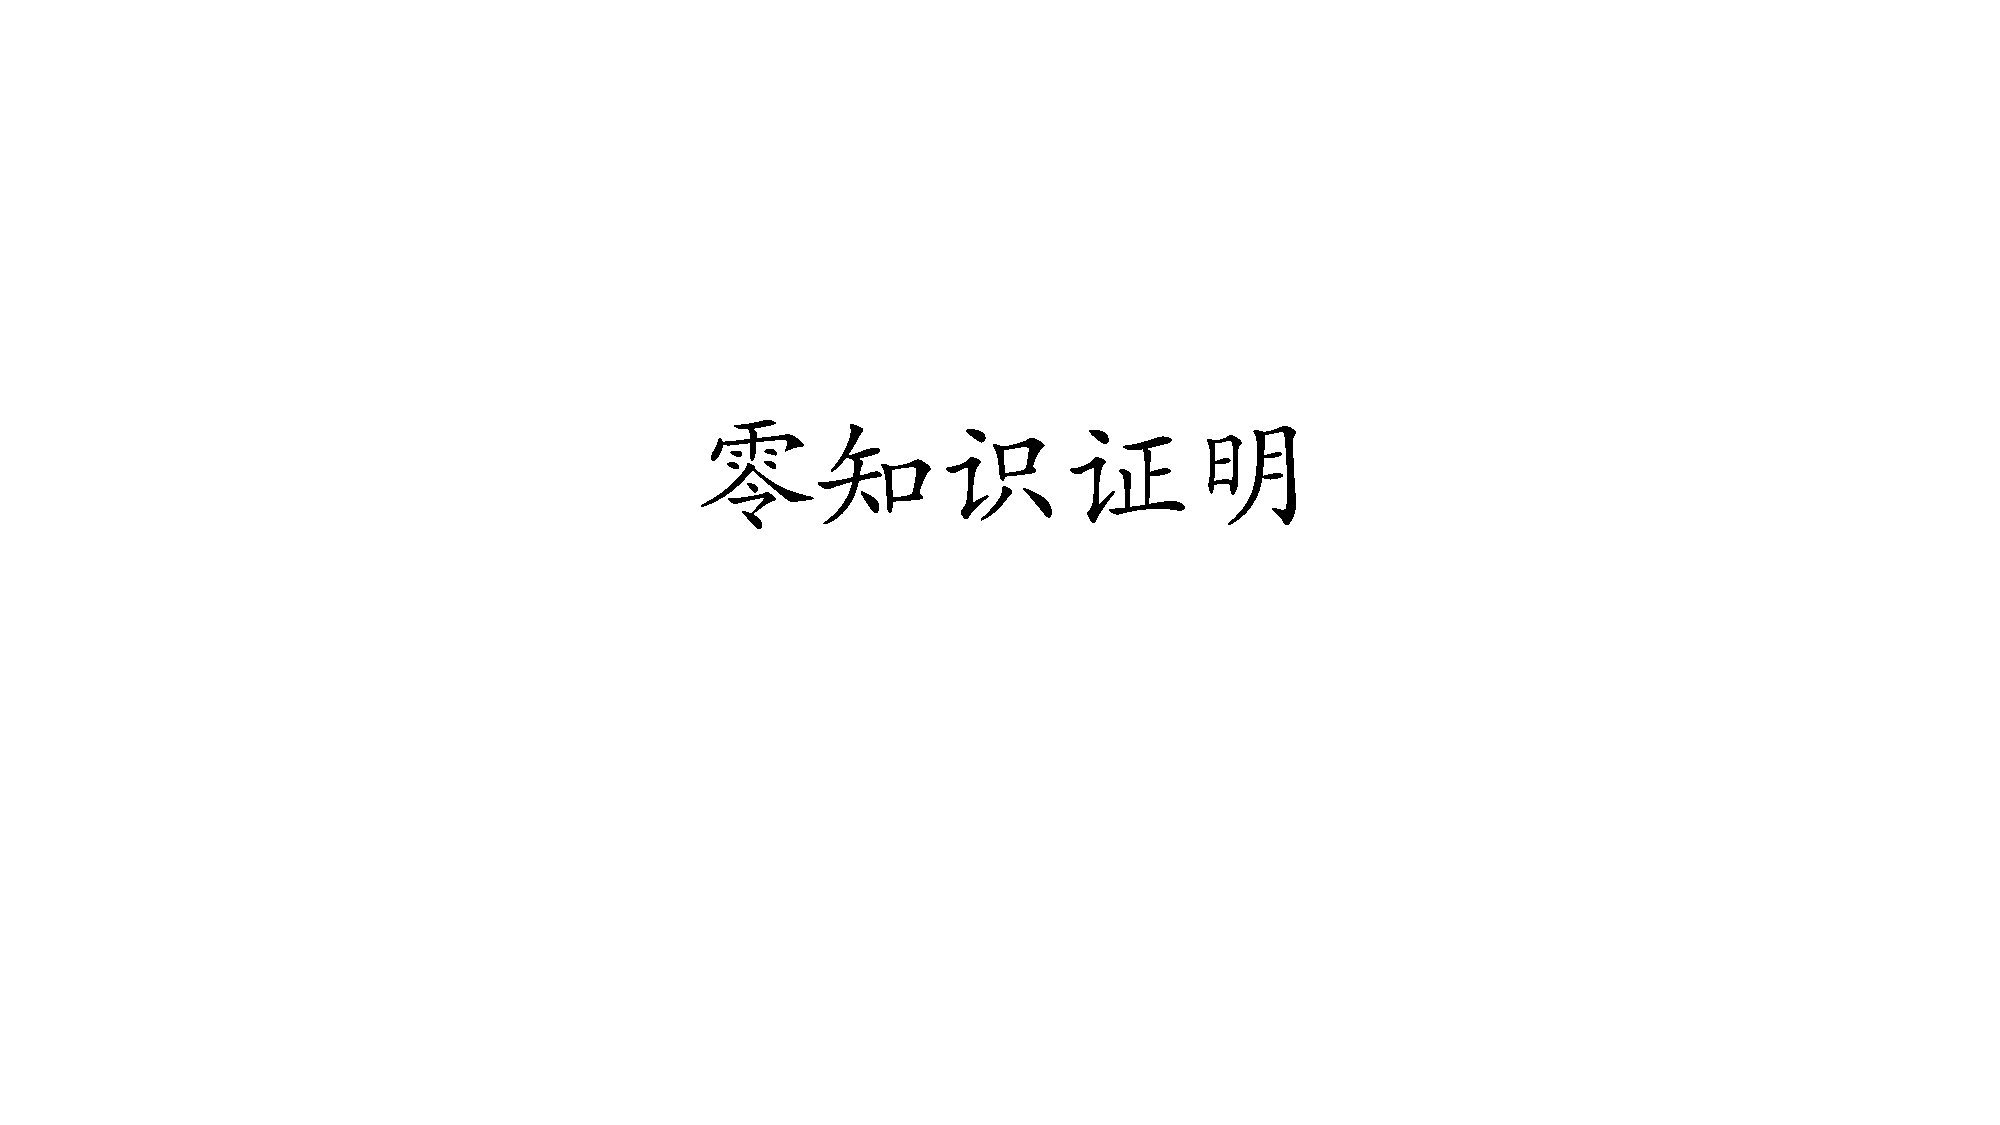
\includepdf[pages=-,nup=1x2]{12-BTC.pdf} 
\section{BTC-比特币引发的思考}
\subsection{哈希指针}
区块链中的哈希指针怎么传播?

指针只和本地机器相关。实际系统中用的只有哈希,指针只是一个形式说法。
\begin{figure}[H]
    \centering
    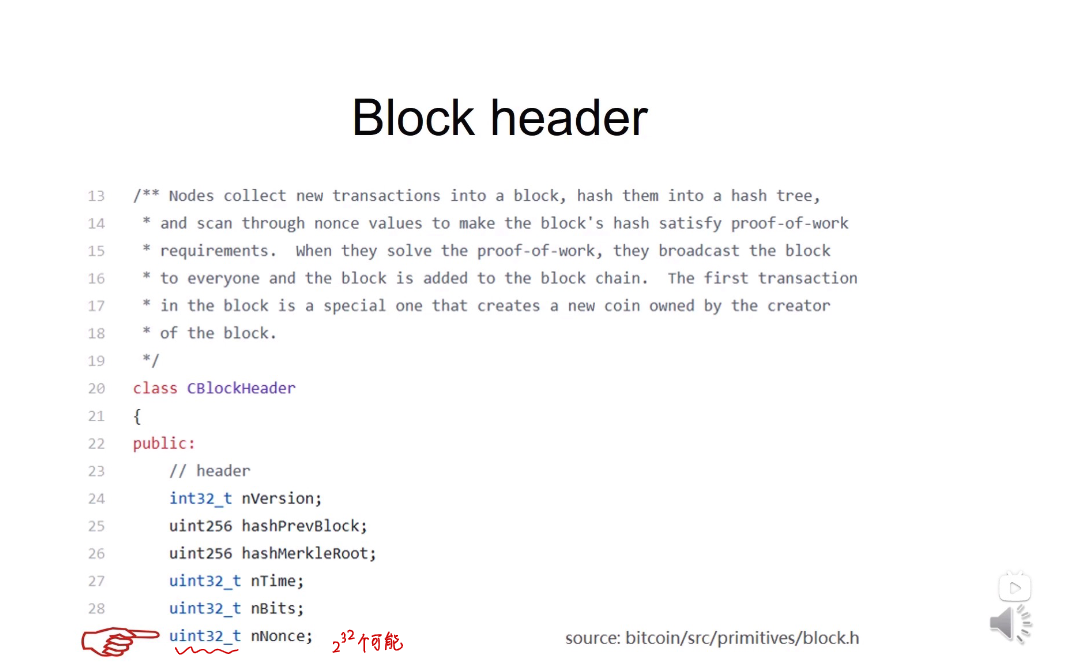
\includegraphics[width=1\textwidth]{./lecture13/img1.png} 
\end{figure}
 
怎么找到区块内容?全节点将这些存在(key, value)数据库中,常用的是levelDB数据库。

\subsection{区块恋}
截断私钥的做法会降低账户的安全性。比特币中的安全和私钥的长度相关,256位,但是如果截断,只需要猜另一半的私钥就能破解。对多个人的账户,不要用截断私钥的方法,用多重签名MULTISIG。

区块恋中可能会造成死钱,UTXO中的死钱是普遍问题。
\subsection{分布式共识}
为什么比特币系统能够绕过分布式共识中那些不可能结论?

严格地说,比特币并没有取得真正意义下的共识。例如分叉。理论和实际有一定距离。

远程服务器连不上,如何区分是垮掉还是运行缓慢?

分布式理论证明在异步(通讯的延迟没有上限)的环境中,不可能区分某台远程服务器是垮掉还是运行缓慢。实际中可以给服务器加一个电话线,可以拨号上网。

\subsection{比特币的稀缺性}
挖矿的收益要大于挖矿的开销。比特币早期挖矿难度低,出块奖励多。

总量固定的东西实际不适合作为货币。一个好的货币要有通货膨胀的功能。

\subsection{量子计算}
量子计算技术离实用还有很大距离。量子计算对传统金融的冲击更大。

比特币中并没有将账户的公钥直接暴露出来,而是用公钥的哈希。即使用量子计算机,也没办法进行哈希的逆运算。从安全角度来看,比特币中的地址用过一次后就不要再用了。即使是公钥,也不要随便泄漏。

\section{ETH-以太坊概述}
以太坊的出块时间变为十几秒。同时改变了mining puzzle,对内存要求高,叫memory hard mining puzzle,限定了ASIC芯片的使用(ASIC resistance)。用权益证明(proof of stake)来替代工作量证明(proof of work)。增加了对智能合约(smart contract)的支持。

BitCoin: decentralized currency, BTC 最小单位Satoshi

Ethereum: decentralized contract, ETH 最小单位Wei

去中心化的货币,可以跨国转账。去中心化的合同,如果合约的签署方来自各国,可以用智能合约。就算是同一个司法管辖权内,司法手段也可能比较麻烦。智能合约的代码一经发布到区块链中,就不可以篡改。

\section{ETH-账户}
A $\rightarrow$ B(10BTC),要说明币的来源。B $\rightarrow$ C(3BTC),不说明的话剩下的7个BTC当成gas费了,所以剩下的币要转给自己另外的账户B $\rightarrow$ B‘(7BTC)。

以太坊采用基于账户的模型(account-based ledger)。A $\rightarrow$ B(10ETH),检查交易的合法性只用检查A账户上的钱是否足够,不用说明币的来源。比特币面临的挑战是double spending attack,以太坊天然能防御这一点。

账户的余额不能随便改,因为账户的余额在全节点中维护。

replay attack,重放攻击,A $\rightarrow$ B(10ETH),假设B是恶意的,再把这个交易广播一次,将A的钱扣了两次。比特币中不会出现repaly attack,因为这会导致double spending。以太坊中加一个nonce,记录交易次数,发布交易时加上这个nonce,整个内容由账户进行签名。系统中会维护账户的余额和nonce值。

以太坊中有两类账户,一类是外部账户externally owner account。外部账户状态有balance、nonce(实际是计数器)。通过公私钥对控制。第二类账户是合约账户smart contract account。合约账户不能主动发起一个交易。合约账户有balance、nonce、code、storage。合约账户可以被调用。

以太坊的创始人Vitalik。以太坊支持合约,要求参与者有稳定的身份。用合约实现金融衍生品(financial derivative)。

\section{ETH-状态树}
以太坊中将账户地址映射到状态,addr $\rightarrow$ state。地址是160bits,一般表示成40个十六进制的数。

\textbf{以太坊中如何证明某个账户的余额是多少?}

比特币中是对一个区块中的几百到几千个交易构成一个新的Merkle tree。而在以太坊中,如果将所有的账户-状态组织成哈希表结果,将账户组织成Merkle tree,这样需要包括的账户数太多。Merkle tree除了证明某个交易在区块中,还有一个作用是保持全节点中内容的一致性,这也是为什么比特币中要将Merkle tree的根哈希值写在块头里。

如果直接将账户-状态构建成一个Merkle tree,问题在于Merkle tree没有提供一个高效的查找和更新的方法。还有一个问题是Merkle tree要不要排序(sorted Merkle tree)?不排序会导致构建Merkle tree是不一样的,算出的根哈希值也不相同。新节点产生是随机的,会插入到Merkle tree中,导致Merkle tree需要更新,可能大半个树需要重构,加入的代价比较大。

trie 字典树,从retrieval中来。分叉数目branching factor。以太坊中是17(加上结束标志位)。trie中地址长度相同,也就是查找长度相同。trie中不会出现碰撞。trie会得到相同的树。更新操作具有局部性,用trie只用访问一个分支。trie的存储会增大。

Patricia tree/trie。经过路径压缩的前缀树。如果新插入一个节点,原来压缩的路径可能会展开。插入的节点的键值分布稀疏,压不压缩效果比较大。例如单词misunderstanding、decentralization、disintermediation(去中间商)。

MPT(Merkle Patricia tree)。把普通指针换成哈希指针。可以计算出根哈希值,写在block header里。根哈希值的作用:防止篡改以及Merkle proof(证明账户余额、证明某个键值不在MPT中)。

以太坊中用的是Modified MPT。合约账户中的存储用的也是MPT。

\textbf{为什么每次改变是新建一个分支而不是直接在原来的MPT中更新数据?}
\begin{figure}[H]
    \centering
    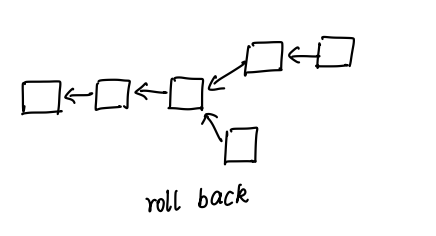
\includegraphics[width=0.4\textwidth]{./lecture16/img1.png} 
\end{figure}
比特币中A $\rightarrow$ B(10BTC),回滚比较容易。以太坊中有智能合约,是图灵完备的,以太坊中如果不保存以前的状态,推算出原来的状态是比较难的,要想支持回滚,必须保存历史状态。

以太坊有三棵树:状态树、交易树、收据树。

状态树中保存的是(key,value)。value要经过序列化(RLP,Recursive Length Prefix)再存储。protocol buffer,简称protobuf,作序列化的库。RLP只支持nested array of bytes,字节数组,可以嵌套。

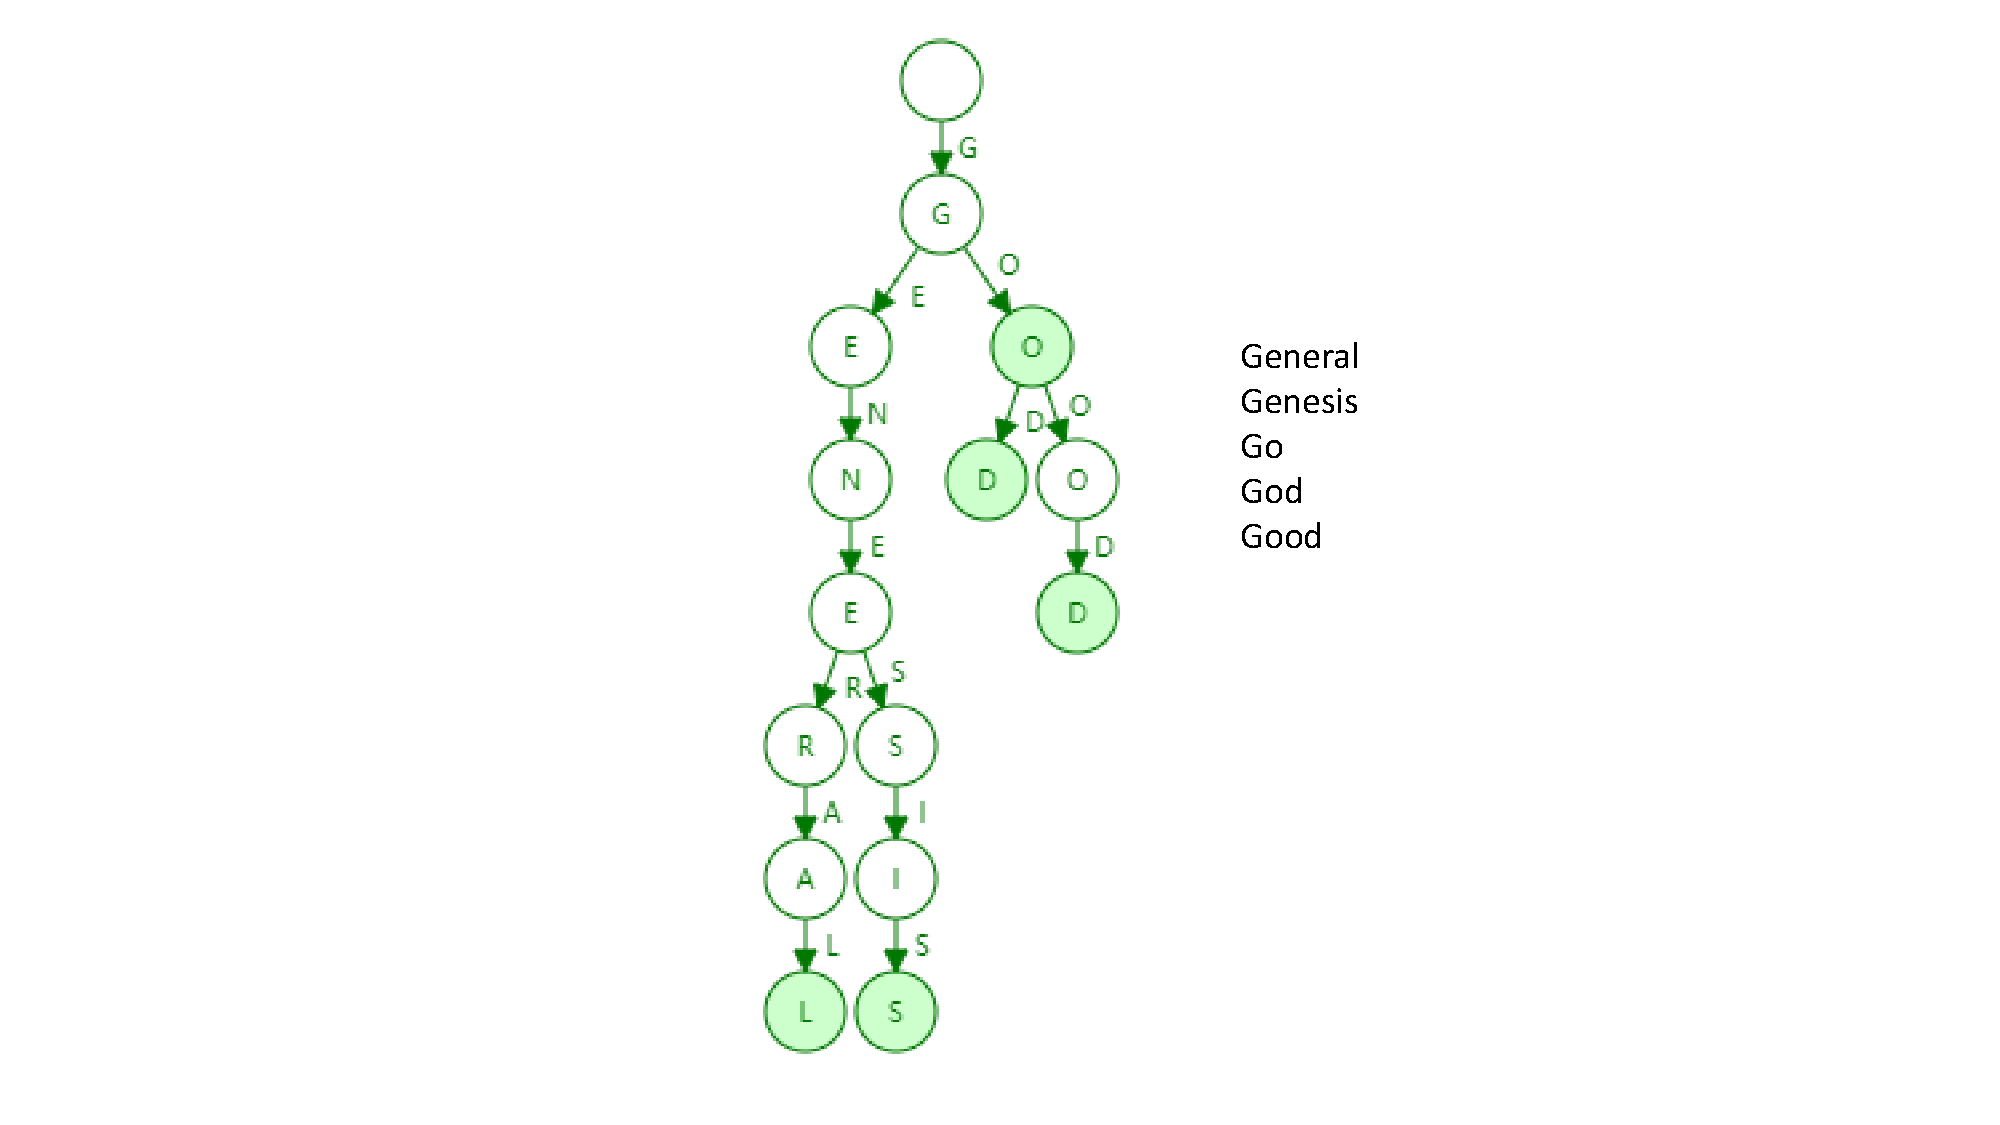
\includepdf[pages=-,nup=1x2]{16-ETH.pdf} 


\end{document}
